%%%%%%%%%%%%%%%%%%%%%%%%%%%%%%%%%%%%%%%%%%%%%%%%%%%%%%%%%%%%%%%%%%%%%%%%%%%%%%%%
%% Plantilla de memoria en LaTeX para la EIF - Universidad Rey Juan Carlos
%%
%% Por Gregorio Robles <grex arroba gsyc.urjc.es>
%%     Grupo de Sistemas y Comunicaciones
%%     Escuela de Ingeniería de Fuenlabrada
%%     Universidad Rey Juan Carlos
%% (muchas ideas tomadas de Internet, colegas del GSyC, antiguos alumnos...
%%  etc. Muchas gracias a todos)
%%
%% La última versión de esta plantilla está siempre disponible en:
%%     https://github.com/gregoriorobles/plantilla-memoria
%%
%% Para obtener PDF, ejecuta en la shell:
%%   make
%% (las imágenes deben ir en PNG o JPG)

%%%%%%%%%%%%%%%%%%%%%%%%%%%%%%%%%%%%%%%%%%%%%%%%%%%%%%%%%%%%%%%%%%%%%%%%%%%%%%%%

\documentclass[a4paper, 12pt]{book}
%\usepackage[T1]{fontenc}

\usepackage[a4paper, left=2.5cm, right=2.5cm, top=3cm, bottom=3cm]{geometry}
\usepackage{times}
\usepackage[utf8]{inputenc}
\usepackage[spanish]{babel} % Comenta esta línea si tu memoria es en inglés
\usepackage{url}
%\usepackage[dvipdfm]{graphicx}
\usepackage{graphicx}
\usepackage{float}  %% H para posicionar figuras
\usepackage[nottoc, notlot, notlof, notindex]{tocbibind} %% Opciones de índice
\usepackage{latexsym}  %% Logo LaTeX
\usepackage{multicol}
\usepackage[table,xcdraw]{xcolor}
\usepackage{array}
\usepackage{longtable}

\title{Memoria del Proyecto}
\author{Nombre del autor}

\renewcommand{\baselinestretch}{1.5}  %% Interlineado

\begin{document}

\renewcommand{\refname}{Bibliografía}  %% Renombrando
\renewcommand{\appendixname}{Apéndice}


%%%%%%%%%%%%%%%%%%%%%%%%%%%%%%%%%%%%%%%%%%%%%%%%%%%%%%%%%%%%%%%%%%%%%%%%%%%%%%%%
% PORTADA

\begin{titlepage}
\begin{center}

\includegraphics[scale=0.6]{img/URJ_logo_Color_POS.png}

\vspace{1.75cm}

\LARGE
ESCUELA DE INGENIERÍA DE FUENLABRADA
\vspace{1cm}

\LARGE
GRADO EN INGENIERÍA DE TECNOLOGÍAS DE TELECOMUNICACIÓN

\vspace{1cm}
\LARGE
\textbf{TRABAJO FIN DE GRADO}

\vspace{2cm}

\Large
EVOLUCIÓN DE LA PARTICIPACIÓN VOLUNTARIA DE PROYECTOS DE SOFTWARE LIBRE:
EVIDENCIAS DE DEBIAN

\vspace{2cm}

\large
Autor : Pablo Cabeza Portalo \\
Tutor : Dr. Gregorio Robles\\

\vspace{1cm}

\large
Curso académico 2023/2024

\end{center}
\end{titlepage}

\newpage
\mbox{}
\thispagestyle{empty} % para que no se numere esta pagina



%%%%%%%%%%%%%%%%%%%%%%%%%%%%%%%%%%%%%%%%%%%%%%%%%%%%%%%%%%%%%%%%%%%%%%%%%%%%%%%%
%%%% Para firmar
\clearpage
\pagenumbering{gobble}
\chapter*{}

\vspace{-4cm}
\begin{center}
\LARGE
\textbf{Trabajo Fin de Grado}

\vspace{1cm}
\large
Reproducción de un trabajo con evidencias de Debian

\vspace{1cm}
\large
\textbf{Autor :} Pablo Cabeza Portalo \\
\textbf{Tutor :} Dr. Gregorio Robles

\end{center}

\vspace{1cm}
La defensa del presente Proyecto Fin de Carrera se realizó el día \qquad$\;\,$ de \qquad\qquad\qquad\qquad \newline de 2024, siendo calificada por el siguiente tribunal:


\vspace{0.5cm}
\textbf{Presidente:}

\vspace{1.2cm}
\textbf{Secretario:}

\vspace{1.2cm}
\textbf{Vocal:}


\vspace{1.2cm}
y habiendo obtenido la siguiente calificación:

\vspace{1cm}
\textbf{Calificación:}


\vspace{1cm}
\begin{flushright}
Fuenlabrada, a \qquad$\;\,$ de \qquad\qquad\qquad\qquad de 2024
\end{flushright}

%%%%%%%%%%%%%%%%%%%%%%%%%%%%%%%%%%%%%%%%%%%%%%%%%%%%%%%%%%%%%%%%%%%%%%%%%%%%%%%%
%%%% Dedicatoria

\chapter*{}
\pagenumbering{Roman} % para comenzar la numeracion de paginas en numeros romanos
\begin{flushright}
\textit{Dedicado a \\
mi familia, mis amigos y a mi pareja.}
\end{flushright}

%%%%%%%%%%%%%%%%%%%%%%%%%%%%%%%%%%%%%%%%%%%%%%%%%%%%%%%%%%%%%%%%%%%%%%%%%%%%%%%%
%%%% Agradecimientos

\chapter*{Agradecimientos}
%\addcontentsline{toc}{chapter}{Agradecimientos} % si queremos que aparezca en el índice
\markboth{AGRADECIMIENTOS}{AGRADECIMIENTOS} % encabezado 

Este es el fin de una de las etapas más importantes de mi vida y por ello quiero agradecer a varias personas que me han acompañado en este proceso.
Primero quiero agradecer a mi madre Antonia todo el apoyo que me ha dado en cada una de mis decisiones, tanto personales como académicas. Eres quien me impulsa a lograr mis sueños.
Segundo a mi padre Manuel que siempre ha sido mi ejemplo a seguir. Me ha aportado valores fundamentales como el trabajo y el esfuerzo que han sido imprescindibles para abordar esta carrera.
Gracias a los dos por darme la vida.
También agradecer a mi tutor, Gregorio, por darme este proyecto, tener paciencia  y ayudarme en todo cuanto pudo para desarrollarlo.
Por último, quiero agradecer a esa persona tan especial que conocí en esta universidad y que me dio la confianza y la fuerza necesaria para lograr mis metas. 
Paula, gracias por ser mi compañera de viaje y por aparecer en el momento que mas lo necesitaba. Hemos afrontado este desafío juntos y sin ti no hubiera sido igual.


%%%%%%%%%%%%%%%%%%%%%%%%%%%%%%%%%%%%%%%%%%%%%%%%%%%%%%%%%%%%%%%%%%%%%%%%%%%%%%%%
%%%% Resumen

\chapter*{Resumen}
%\addcontentsline{toc}{chapter}{Resumen} % si queremos que aparezca en el índice
\markboth{RESUMEN}{RESUMEN} % encabezado

Este proyecto se basa en un estudio sobre la evolución de la distribución más importante de Linux llamada Debian, la cual es de software libre. Partimos de un estudio anterior titulado ``Evolution of Volunteer Participation in Libre Software Projects: Evidence from Debian''~\cite{robles05:_debian} del cual se ha realizado una réplica veinte años después. 

El objetivo principal es responder a una serie de preguntas planteadas en dicho estudio las cuales nos darán la información necesaria para comprender como evoluciona Debian y si cumplen las tendencias estudiadas en el artículo anterior.
Dichas preguntas son: \textbf{¿Cuántos mantenedores tiene Debian y cómo cambia este número con el tiempo?, ¿Existe una tendencia hacia la formación de equipos de mantenedores?, ¿Cuántos mantenedores de versiones anteriores permanecen activos?, ¿Cuál es el aporte de los mantenedores que permanecen en versiones posteriores?, ¿Qué sucede con los paquetes mantenidos por los mantenedores que abandonan el proyecto? y ¿Los paquetes más importantes y de uso común son mantenidos por mantenedores más experimentados?}.

Para obtener las conclusiones deseadas se ha pasado por las etapas de \textbf {descarga de releases de Debian, análisis de los paquetes de los releases, creación de diagrama entidad-relación, creación de bases de datos junto con sus tablas SQL, parseo de la información de cada paquete, obtención de gráficos sobre la información, creación de \emph{queries} e inserción de la información en la base de datos}.

Para ello se usan tecnologías tales como \textbf {Pycharm y MySQL Worckbench}.
En ellas necesitamos el uso de lenguajes de programación tales como \textbf {Python y SQL} junto con librerías de Python como \textbf {MySQL Connector o Matplotlib}.


%%%%%%%%%%%%%%%%%%%%%%%%%%%%%%%%%%%%%%%%%%%%%%%%%%%%%%%%%%%%%%%%%%%%%%%%%%%%%%%%
%%%% Resumen en inglés

\chapter*{Summary}
%\addcontentsline{toc}{chapter}{Summary} % si queremos que aparezca en el índice
\markboth{SUMMARY}{SUMMARY} % encabezado
This project is based on a study about the evolution of the most important Linux distribution called Debian, which is free software. We started from a previous study called "Evolution of Volunteer Participation in Libre Software Projects: Evidence from Debian"~\cite{robles05:_debian}, which has been replicated twenty years later.

The main objective is to answer the questions raised in that study, which will provide us with the necessary information to understand how Debian evolves and if it follows the trends from the previous study.
These questions are: \textbf{How many maintainers does Debian have and how does this number change over time?, Is there a pattern of creating maintainer teams?, How many maintainers from previous versions remain active?, What is the contribution of maintainers who stay in later versions?, What happens to the packages maintained by maintainers who leave the project?,Are the most important and commonly used packages maintained by more experienced maintainers?}

To get the results we want, we have gone through the stages of \textbf{downloading Debian releases, analyzing the packages of the releases, creating an entity-relationship diagram, creating databases and their SQL tables, parsing the information of each package, obtaining graphs on the information, creating queries, and inserting the information into the database}.

For this purpose, technologies such as \textbf{PyCharm and MySQL Workbench} are used.
In them, we use programming languages like \textbf{Python and SQL} and Python libraries like \textbf{MySQL Connector and Matplotlib}.


%%%%%%%%%%%%%%%%%%%%%%%%%%%%%%%%%%%%%%%%%%%%%%%%%%%%%%%%%%%%%%%%%%%%%%%%%%%%%%%%
%%%%%%%%%%%%%%%%%%%%%%%%%%%%%%%%%%%%%%%%%%%%%%%%%%%%%%%%%%%%%%%%%%%%%%%%%%%%%%%%
% ÍNDICES %
%%%%%%%%%%%%%%%%%%%%%%%%%%%%%%%%%%%%%%%%%%%%%%%%%%%%%%%%%%%%%%%%%%%%%%%%%%%%%%%%

% Las buenas noticias es que los índices se generan automáticamente.
% Lo único que tienes que hacer es elegir cuáles quieren que se generen,
% y comentar/descomentar esa instrucción de LaTeX.

%%%% Índice de contenidos
\tableofcontents 
%%%% Índice de figuras
\cleardoublepage
%\addcontentsline{toc}{chapter}{Lista de figuras} % para que aparezca en el indice de contenidos
\listoffigures % indice de figuras
%%%% Índice de tablas
%\cleardoublepage
%\addcontentsline{toc}{chapter}{Lista de tablas} % para que aparezca en el indice de contenidos
%\listoftables % indice de tablas


%%%%%%%%%%%%%%%%%%%%%%%%%%%%%%%%%%%%%%%%%%%%%%%%%%%%%%%%%%%%%%%%%%%%%%%%%%%%%%%%
%%%%%%%%%%%%%%%%%%%%%%%%%%%%%%%%%%%%%%%%%%%%%%%%%%%%%%%%%%%%%%%%%%%%%%%%%%%%%%%%
% INTRODUCCIÓN %
%%%%%%%%%%%%%%%%%%%%%%%%%%%%%%%%%%%%%%%%%%%%%%%%%%%%%%%%%%%%%%%%%%%%%%%%%%%%%%%%

\cleardoublepage
\chapter{Introducción}
\label{sec:intro} % etiqueta para poder referenciar luego en el texto con~\ref{sec:intro}
\pagenumbering{arabic} % para empezar la numeración de página con números

Vivimos en un mundo totalmente digitalizado en el que la presencia de ordenadores está a la orden del día. Con esto no nos referimos únicamente a ordenadores de escritorio. A diario interactuamos con una amplia gama de dispositivos compuestos por ordenadores camuflados. Desde electrodomésticos inteligentes pasando por coches modernos hasta en tarjetas de crédito. Estos tienen incorporados ordenadores pequeños pero potentes que realizan una serie de tareas para el beneficio y la mejora de la vida humana.

En la mayoría de estos ordenadores de uso cotidiano, como portátiles o móviles, se aloja un Sistema Operativo. Un Sistema Operativo es el “intermediario” entre el usuario y el hardware del ordenador a partir de software. Gestiona los recursos del hardware proporcionando una interfaz al usuario. De esta forma pueden interactuar con dicho ordenador. 
Algunos de los sistemas operativos más usados son: iOS, Android, MacOS, Microsoft Windows o Linux. 

Linux es un sistema operativo de código abierto el cual es gratuito para cualquier usuario que quiera adoptarlo en su computadora. Este consta de muchas distribuciones. Las distribuciones son versiones del Sistema Operativo de Linux desarrolladas por diferentes individuos, equipos o empresas para mejorar la experiencia de los usuarios.

Una de estas distribuciones es “Debian” y es sobre la que tratará este estudio.
Debian es un Sistema Operativo que trabaja con el Kernel (núcleo) de Linux y ha ido aportando distintas versiones desde 1993. 
Treinta años después nos preguntamos ciertas cosas como, ¿Los individuos que trabajaban en las primeras versiones siguen actualizando Debian? ¿Se trabaja individualmente o por equipos? ¿Cuántos paquetes sacan en cada versión? ¿Qué ocurre con ellos? Todo esto lo veremos a continuación.



\section{Contexto}
\label{sec:contexto}



\subsection{Proyecto Debian}
\label{subsec:proyecto debian}

El Proyecto Debian está formado por un grupo de voluntarios a nivel mundial que trabajan para producir una distribución del Sistema Operativo Linux basada en `software libre'.

Con el término `software libre' no nos referimos a su coste. Este va enfocado a la `libertad real' dentro del software, es decir, `software de código abierto'.
Esto significa que cualquier usuario puede acceder al código fuente para estudiarlo, revisarlo, modificarlo o distribuirlo sin restricción alguna.

Debian es la distribución de Linux más relevante sin fines comerciales.
En su comienzo, fue la única abierta a la participación de diferentes usuarios que quisieran aportar al proyecto con su trabajo.

Con el tiempo fue asentando un gran conjunto de directrices y procedimientos para el empaquetamiento y distribución de software. Esto les sirvió para poder alcanzar los estándares de calidad requeridos y con ello asegurar su buen funcionamiento.

\subsection{Versiones Debian}
\label{subsec:versiones debian}

Debian ha publicado varias versiones desde 1993 las cuales explicaremos a continuación:

\begin{itemize}

	\item \textbf {Versiones 0.x (1993 - 1995):} estas versiones fueron las primeras y más rudimentarias pero dieron lugar a la creación de Debian gracias a su creador \textbf {Ian Murdock}.
	\begin{itemize}
		\item \textbf {Debian 0.01 hasta 0.90.}
		\item \textbf {Debian 0.91:} disponía de un sencillo sistema de empaquetamiento que permitía instalar y desinstalar paquetes.
		\item \textbf {Debian 0.93R5:}  se asignaron responsabilidades de cada paquete a cada uno de los desarrolladores. Se comenzó a usar el administrador de paquetes \textbf {dpkg} para la instalación de paquetes después de la instalación del sistema.
		base.
	\end{itemize}
	\item \textbf {Versiones 1.x (1996 - 1997):} \textbf{Bruce Perens} fue designado como líder del proyecto después de que Ian lo designara.
	\begin{itemize}
		\item \textbf {Debian 1.0:} esta versión nunca fue publicada debido a una confusión al distribuir una versión en desarrollo con el nombre equivocado de Debian 1.0 que daría problemas en ejecución.
		\item \textbf {Debian 1.1 Buzz: } es la primera versión de Debian con un nombre en clave sacado de las películas de \textbf {`Toy Story'}.
		\item \textbf {Debian 1.2 Rex: } esta versión estaba completamente en formato \textbf{ELF} y usaba el núcleo (kernel) Linux 2.0.
		
		El formato \textbf{ELF} (Executable and Linkable Format) es un estándar. Se usa en sistemas operativos tipo \textbf{UNIX} (como Linux). Sirve para organizar y manejar archivos ejecutables, bibliotecas compartidas y otros objetos binarios.
		\item \textbf {Debian 1.3 Bo}.
	\end{itemize}
	\item \textbf {Versiones 2.x (1998 - 2000):} \textbf{Ian Jackson} pasó a ser el líder del proyecto.
	\begin{itemize}
		\item \textbf {Debian 2.0 Hamm: }fue la primera versión multiplataforma de Debian. Agregó soporte para arquitecturas de la serie \textbf{Motorola 68000}.
		\item \textbf {Debian 2.2 Potato: }agregó soporte para las arquitecturas  PowerPC y ARM (CPU's de arquitectura RISC creadas por diferentes empresas).
	\end{itemize}
	\item \textbf {Versiones 3.x (2002 -2005):}
	\begin{itemize}
		\item \textbf {Debian 3.0 Woody: }se agregaron más arquitecturas a esta versión y fue la primera en usar \textbf {software criptográfico}. Este se usa para codificar información y mantener la transferencia segura de datos.
		\item \textbf {Debian 3.1 Sarge: }incluye un nuevo instalador llamado \textbf {debian-installer}. Contiene detección automática de hardware, instalación sin supervisión y está traducido a más de treinta idiomas.
	\end{itemize}
	\item \textbf {Debian 4.0 Etch (2007):} se añadieron mejoras como un instalador gráfico o la verificación criptográfica de los paquetes descargados entre otras.
	\item \textbf {Debian 5.0 Lenny (2009):} añadió la arquitectura \textbf {ARM EABI} para dar soporte a los nuevos procesadores \textbf {ARM}.
	\item \textbf {Debian 6.0 Squeeze: }con esta versión fue la primera vez que una distribución de Linux se extendía para permitir también el uso de un núcleo no Linux.
	\item \textbf {Debian 7.0 Wheezy (2011):} se introdujo el soporte de \textbf {multiarquitectura}. Esto permitía que los usuarios instalaran en una misma máquina paquetes de múltiples arquitecturas.
	\item \textbf {Debian 8 Jessie (2013):} trajo importantes mejoras de seguridad, como un nuevo kernel que solucionaba varias vulnerabilidades (como \textbf {ataques de enlace simbólico}).
	\item \textbf {Debian 9 Stretch (2015):} se introdujeron paquetes para la depuración a través de un repositorio nuevo en el archivo. Facilitaría el proceso de depuración y solución de problemas relacionados con esos paquetes.
	\item \textbf {Debian 10 Buster (2019):} incluyó por primera vez un marco de control de acceso obligatorio. Restringe las acciones que pueden realizar los programas, limitando su acceso a ciertos recursos del sistema, como archivos, directorios, redes, etc.
	\item \textbf {Debian 11 Bullseye (2021):} introduce un nuevo paquete, ipp-usb, que utiliza el protocolo IPP-over-USB, independiente del fabricante y soportado por muchas impresoras actuales. Esto permite que un dispositivo USB sea tratado como un dispositivo de red.
	
		
\end{itemize}
	
\subsection{ Evolución de la Participación Voluntaria en Proyectos de Software Libre: Evidencia de Debian}
\label{subsec:articulo debian}

Este proyecto es la réplica del articulo \textbf {Evolución de la Participación Voluntaria en Proyectos de Software Libre:
Evidencia de Debian}~\cite{robles05:_debian}.

En este 
artículo se analiza la evolución en el tiempo de los recursos humanos de 
uno de los proyectos de software libre más grandes y complejos 
compuesto principalmente por voluntarios, el proyecto Debian.

Se realiza una investigación 
cuantitativa de datos de casi siete años, estudiando cómo la participación 
de voluntarios ha afectado al software lanzado por el proyecto y a la 
propia comunidad de desarrolladores.

Los resultados que se obtuvieron fueron los siguientes:
\begin{itemize}
	\item \textbf {Número de \emph{maintainers} de cada versión}: se llegó a la conclusión de que aumenta el número de maintainers con el tiempo. También aumenta el número de paquetes por maintainer por lo que se supuso una mayor eficiencia de los maintainers debido a mejoras en las herramientas.
	
	\begin{table}[]
		\begin{tabular}{|l|r|r|r|r|}
			\hline
			Fecha        & Release & Nº Maintainers & Paquetes & Paquetes/Maintainer \\ \hline
			Julio 98     & 2.0     & 217           & 1.101    & 5,1                 \\ \hline
			Marzo 99    & 2.1     & 297           & 1.559    & 5,2                 \\ \hline
			Agosto 00   & 2.2     & 453           & 2.601    & 5,7                 \\ \hline
			Julio 02     & 3.0     & 859           & 5.119    & 6,0                 \\ \hline
			Diciembre 04 & (3.1)   & 1237          & 7.786    & 6,3                 \\ \hline
		\end{tabular}
		\caption{Nº de maintainers, paquetes y paquetes por maintainer}
	\end{table}
	
	\item \textbf {¿Existe una tendencia hacia la formación de equipos de 
	mantenedores?}: los resultados que se obtuvieron marcan una clara tendencia a la formación de los mismos.
	
	\begin{table}[h]
		\begin{tabular}{|l|r|r|r|r|}
			\hline
			Fecha        & Release & Paquetes en Grupo & Paquetes de Quality Control & Porcentaje \\ \hline
			Julio 98     & 2.0     & 14             & 14                       & 1,3\%      \\ \hline
			Marzo 99    & 2.1     & 21             & 11                       & 1,4\%      \\ \hline
			Agosto 00   & 2.2     & 46             & 31                       & 1,8\%      \\ \hline
			Julio 02     & 3.0     & 101            & 71                       & 2,2\%      \\ \hline
			Diciembre 04 & (3.1)   & 599            & 194                      & 7,4\%      \\ \hline
		\end{tabular}
		\caption{Nº de grupos, paquetes de los grupos y porcentaje de paquetes asociados a grupos}
	\end{table}
	
	\item \textbf {Seguimiento de los mantenedores restantes de Debian}: se estudió el número de maintainers que había en la primera versión y como disminuye con el paso del tiempo debido a que abandonan el proyecto. 
	
	\begin{table}[h]
		\begin{tabular}{|l|r|r|r|r|}
			\hline
			Fecha        & Release & Maintainers 1ª versión & Paquetes & Paquetes/Maintainer \\ \hline
			Julio 98     & 2.0     & 216                     & 1.101       & 5,1                 \\ \hline
			Marzo 99    & 2.1     & 207                     & 1.086       & 5,2                 \\ \hline
			Agosto 00   & 2.2     & 188                    & 1.040       & 5,5                 \\ \hline
			Julio 02     & 3.0     & 147                    & 870       & 5,9                 \\ \hline
			Diciembre 04 & (3.1)   & 121                    & 729      & 6                   \\ \hline
		\end{tabular}
		\caption{Nº de maintainers de la 1ª versión, paquetes y paquetes por maintainer}
	\end{table}
	
	\item \textbf {Investigar la experiencia del mantenedor}: se estudió si los mantenedores más experimentados tenían asociados mayor cantidad de paquetes pero resultó ser una proporción igualada. Aunque se debería estudiar más a fondo.
	
	\item \textbf {Paquetes de mantenedores que abandonaron el proyecto}: se observó que se asignaban los paquetes a otro maintainer cuando abandonaba el proyecto y tenía paquetes asociados. 
	
	\item \textbf {Experiencia e importancia}: se llegó a la conclusión de que los paquetes con mayor número de instalaciones y más usados se asignaban a maintainers más experimentados.
	
	
\end{itemize}

Este articulo se publicó en 2005. A día de hoy, se han publicado ocho versiones nuevas de de Debian y por ello podemos realizar un estudio actualizado de dicha distribución. Con la aportación de nuevos datos que ayuden a manejar una mayor exactitud en las conclusiones y a plantear nuevas cuestiones sobre Debian.

\section{Estructura de la memoria}
\label{sec:estructura}

A continuación se exponen los capítulos en los que se organiza esta memoria y los puntos clave tratados en cada uno de ellos:


\begin{itemize}
  \item \textbf {Capítulo 1: Introducción.} Se explica el contexto de Debian y las diferentes versiones distribuidas a lo largo de su historia.
  
  \item \textbf {Capítulo 2: Objetivos.} Se especifica cuales son los objetivos parciales para lograr el objetivo general.
  
  \item \textbf {Capítulo 3: Estado del arte.} Se muestran y explican las diferentes tecnologías usadas para la realización de dicho proyecto.
  
  \item \textbf {Capítulo 4: Diseño e implementación.} Se muestran las diferentes etapas que se han seguido en este proyecto a detalle.
  
  \item \textbf {Capítulo 5: Experimentos y validación.} Se indica el proceso seguido para alcanzar los diferentes objetivos usando diferentes tecnologías.
  
  \item \textbf {Capítulo 6: Resultados.} Se muestran los diferentes resultados de estos experimentos. También se comentan los diferentes patrones o tendencias procedentes del análisis de dichos resultados.
  
  \item \textbf {Capítulo 7: Conclusiones.} Se observan los resultados obtenidos y se comparan con lo que se esperaba obtener. Se realizan una serie de deducciones tras el tratamiento y el análisis de los datos. Se aplican los conocimientos adquiridos en la carrera y se plantean nuevas lineas de investigación.
  
\end{itemize}





%%%%%%%%%%%%%%%%%%%%%%%%%%%%%%%%%%%%%%%%%%%%%%%%%%%%%%%%%%%%%%%%%%%%%%%%%%%%%%%%
%%%%%%%%%%%%%%%%%%%%%%%%%%%%%%%%%%%%%%%%%%%%%%%%%%%%%%%%%%%%%%%%%%%%%%%%%%%%%%%%
% OBJETIVOS %
%%%%%%%%%%%%%%%%%%%%%%%%%%%%%%%%%%%%%%%%%%%%%%%%%%%%%%%%%%%%%%%%%%%%%%%%%%%%%%%%

\cleardoublepage % empezamos en página impar
\chapter{Objetivos} % título del capítulo (se muestra)
\label{chap:objetivos} % identificador del capítulo (no se muestra, es para poder referenciarlo)



\section{Objetivo general} % título de sección (se muestra)
\label{sec:objetivo-general} % identificador de sección (no se muestra, es para poder referenciarla)

Este proyecto de fin de grado se basa en el análisis de los lanzamientos, paquetes y mantenedores presentes en la evolución de la distribución Debian a lo largo de su historia. 

Se busca conocer, para cada versión (\textbf{release}), la evolución en el número de personas y equipos que lo mantienen,  cuántos de ellos siguen en releases posteriores y qué ocurre con los paquetes de un mantenedor si este abandona el proyecto. Se ha podido llevar a cabo gracias al estudio de diferentes paquetes de datos aportados por Debian\footnote{\url{https://www.debian.org/releases/}} en su página oficial.
De esta forma se obtienen las diferencias y similitudes necesarias para la comparación de los releases de forma que se pueda comprender su evolución.


\section{Objetivos específicos}
\label{sec:objetivos-especificos}

Para poder llevar a cabo dicho objetivo se requiere: 

\begin{itemize}
	\item \textbf {Diseñar el diagrama entidad relación.} Se comprenden los diferentes campos que conforman un paquete y se crea un diagrama para el posterior diseño de la base de datos que los alojará.
	.
	\item \textbf {Crear la base de datos.} Se crea una base de datos con un buen diseño (basada en el diagrama anterior) para poder lanzar \textbf {Queries} con las que se obtienen la información que se requiere.
	
	\item \textbf {Inserción de los datos.} Se crea un script para parsear los datos de los paquetes e insertarlos en sus respectivas tablas junto a sus relaciones con otras tablas..
	
	\item \textbf {Formular las queries.} Se analiza la información que se quiere extraer de la base de datos y se crean las llamadas necesarias para obtenerla.
	
	
	\item \textbf {Crear las tablas y gráficas.} Con la información obtenida se crean diferentes tablas y gráficas para ayudar a la comprensión de los datos de forma visual.
\end{itemize}


\section{Planificación temporal}
\label{sec:planificacion-temporal}

En el Diagrama de la Figura~\ref{fig:diagrama_gantt} se visualizan las diferentes tareas realizadas junto con la organización en días de las mismas. 

Primero se marcaron los objetivos junto con las tecnologías a usar en este proyecto.
Más tarde se realizó un análisis de los diferentes paquetes para poder crear el diagrama, el diseño de la base de datos y sus tablas correspondientes.
Realizamos el parseo de las diferentes datos del paquete para poder insertarlos correctamente en la base de datos.
La inserción de los datos fue lo más problemático en este proyecto. Cada release consta de muchos paquetes en los cuales hay que parsear, extraer e insertar todos los datos. Este estudio se realiza sobre 11 releases. Al tratarse de tanto volumen de datos, el tiempo de ejecución fue elevado. Al comprobar las bases de datos y hallar errores, se insertaban de nuevo los datos por lo que esto fue lo más complejo del proyecto.

Finalmente se realizaron una serie de llamadas SQL (queries) con las que extraer la información necesaria para el proyecto junto con sus gráficas para obtener dicha información de forma visual.

Con ello pudimos obtener conclusiones sobre el estudio de estos datos y comenzar con la redacción de la memoria.

El Dr. Gregorio Robles, mi tutor, me propuso dicho proyecto en noviembre de 2023 y el tiempo desempeñado en él ha sido de 4h diarias reflejadas en los días laborales, de lunes a viernes. En los meses de abril y mayo se intensifico mi desempeño a 6h diarias para desarrollar la memoria con la mayor dedicación posible.

\begin{figure}
	\centering
	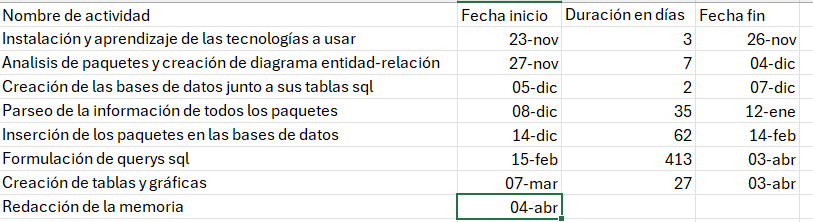
\includegraphics[width=17cm, keepaspectratio]{img/Gantt.png}
	\caption{Diagrama de Gantt}
	\label{fig:diagrama_gantt}
\end{figure}

%%%%%%%%%%%%%%%%%%%%%%%%%%%%%%%%%%%%%%%%%%%%%%%%%%%%%%%%%%%%%%%%%%%%%%%%%%%%%%%%
%%%%%%%%%%%%%%%%%%%%%%%%%%%%%%%%%%%%%%%%%%%%%%%%%%%%%%%%%%%%%%%%%%%%%%%%%%%%%%%%
% ESTADO DEL ARTE %
%%%%%%%%%%%%%%%%%%%%%%%%%%%%%%%%%%%%%%%%%%%%%%%%%%%%%%%%%%%%%%%%%%%%%%%%%%%%%%%%

\cleardoublepage
\chapter{Estado del arte}
\label{chap:estado}
En este capítulo mencionamos las diferentes tecnologías  usadas en este proyecto sin las que no hubiera sido posible su realización.
 

\section{Python 3.12.0} 
\label{sec:python}
\textbf{Python}~\cite{oracle:_python} es un lenguaje de programación orientado a objetos de alto nivel con una sintaxis fácil de interpretar y leer. Tiene un amplio uso en computación científica, desarrollo web y automatización.

\textbf{Peter Norvig}, director de investigación de Google afirma que `Python ha sido una parte importante de Google desde el principio, y permanece así a medida que el sistema crece y evoluciona'.

Al ser un lenguaje popular tiene una mayor selección de bibliotecas, lo que ahorra a un desarrollador cantidades increíbles de tiempo y esfuerzo. También tiene más tutoriales y documentación. Esto aumenta las probabilidades de encontrar soluciones a los problemas.

Una curiosidad del lenguaje es que la empresa de mayor emprendimiento de la `inteligencia artificial'  \textbf{ Open AI\footnote{\url{https://platform.openai.com/docs/libraries/python-library}}} está diseñada con Python en gran parte y sus bibliotecas son públicas para su uso.

En la figura~\ref{fig:evolucion_python} podemos observar que Python es el lenguaje más usado del mundo según sus últimos datos en 2019~\cite{statista:_tecnología}.

\begin{figure}
	\centering
	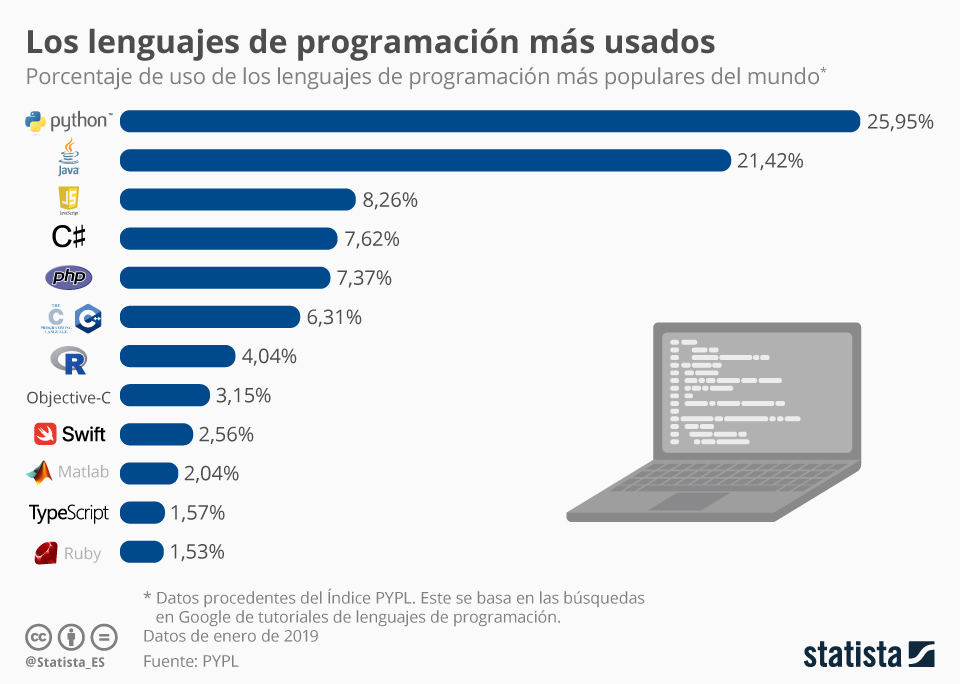
\includegraphics[width=14cm, keepaspectratio]{img/ev_python.jpeg}
	\caption{Lenguajes de programación más usados - Fuente: Guadalupe Moreno.}
	\label{fig:evolucion_python}
\end{figure}

\section{MySQL Connector} 
\label{sec:mysqlconnector}
Esta es la librería más importante de Python para poder desarrollar este proyecto.
MySQL Connector/Python~\cite{mysql:_connectors} permite a los programas de Python acceder a las bases de datos MySQL, utilizando una API que cumple con la Especificación de API de Base de Datos de Python.
Sus funciones más destacadas e importantes son:
\begin{enumerate}
	\item \textbf{Conexión a la base de datos: }con la función \textbf{mysql.connector.connect().}
	\item \textbf{Ejecución de consultas SQL: }con la función \textbf{cursor.execute().}
	\item \textbf{Recuperación de resultados: }con la función \textbf{cursor.fetchall()}.
	\item \textbf{Inserción, actualización y eliminación de datos: }con consultas SQL como INSERT, UPDATE y DELETE, ejecutadas con la función \textbf{cursor.execute().}
	\item \textbf{Gestión de errores: }se capturan y manejan errores en el código Python usando excepciones.
	\item \textbf{Desconexión de la base de datos: }con la función \textbf{connection.close().}
\end{enumerate}

\section{Matplotlib} 
\label{sec:matplotlib}


Matplotlib~\cite{python:_matplotlib} es una librería de \textbf{Python open source}. John Hunter, neurobiólogo, fue su desarrollador inicial en 2002. Su objetivo era visualizar las señales eléctricas del cerebro de personas epilépticas. Por ello intentó replicar las diferentes funcionalidades de MATLAB (gráficas) con Python. 

Matplotlib ha sido mejorado a lo largo del tiempo por numerosos contribuidores de la comunidad open source. Se usa para crear gráficas y diagramas de gran calidad que aportan la visualización de los datos de  forma detallada.

Es posible crear trazados, histogramas, diagramas de barras y cualquier tipo de gráfica como en la Figura~\ref{fig:matplotlib} con unas lineas de código.

Esta librería es particularmente útil para las personas que trabajan con Python o NumPy.

\begin{figure}[hb]
	\centering
	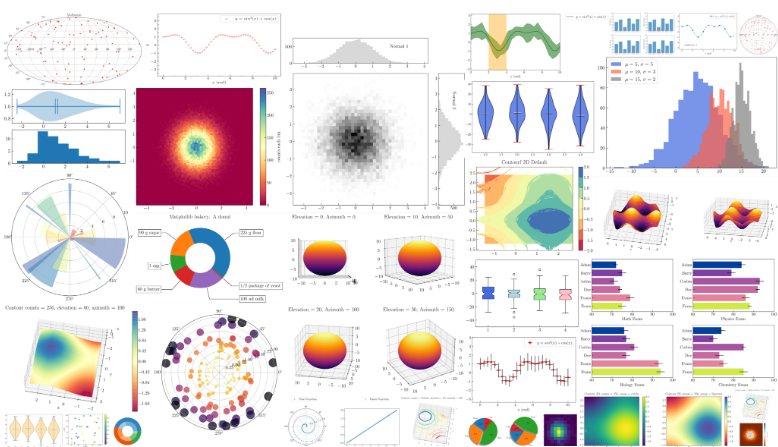
\includegraphics[width=14cm, keepaspectratio]{img/Matplotlib.png}
	\caption{Ejemplos gráficas Matplotlib}
	\label{fig:matplotlib}
\end{figure}

\section{Pycharm} 
\label{sec:pycharm}

PyCharm es el \textbf{IDE}~\cite{python:_pycharm} más popular para Python hasta la fecha. Esta plataforma híbrida se utiliza habitualmente para el desarrollo de aplicaciones en Python por grandes empresas como Twitter, Facebook, Amazon y Pinterest.

Un \textbf{Integrated Development environment (IDE)} o \textbf{Entorno de Desarrollo Integrado (EDI)} es un conjunto de herramientas necesarias para desarrollar software. Incluye un editor y un compilador.


Pycharm es compatible con Windows, Linux y macOS. Además contiene módulos y paquetes que ayudan a los desarrolladores a programar software con Python más rápido y con menos esfuerzo y se puede personalizar para responder a las necesidades específicas de un proyecto.

\begin{figure}[hb]
	\centering
	
\includegraphics[width=14cm, keepaspectratio]{img/pycharm.png}
	\caption{Pycharm}
	\label{fig:pycharm}
\end{figure}

\section{SQL} 
\label{sec:sql}
Es un lenguaje de consulta de bases de datos que \textbf{almacena y procesa información en una base de datos relacional}. 

Una base de datos \textbf{relacional} almacena información en forma de tabla, con filas y columnas que representan diferentes atributos de datos junto con sus relaciones. Con ello se puede \textbf{almacenar, actualizar, eliminar, buscar y recuperar} información de la base de datos.

Es un lenguaje de consulta popular que se usa con frecuencia en todos los tipos de aplicaciones debido a su alta integración con el resto de lenguajes tales como \textbf{Java, Python, C\#, PHP, etc}.

\section{MySQL WorkBench} 
\label{sec:mysqlworkbench}

Es una herramienta visual ideal para \textbf{modelar, diseñar y administrar bases de datos MySQL} junto con el uso de código MySQL.

Se trata de una herramienta gráfica que fue creada por la compañía Oracle.
Es un programa de cliente que, a través de un entorno de desarrollo integrado, facilita la creación, consulta y administración de bases de datos~\cite{mysql:_workbench}. 

Este software tiene múltiples funcionalidades como:
\begin{itemize}
	\item \textbf {Modelado de datos}: diseñar, modelar, gestionar y generar bases de datos de forma visual. 
	\item \textbf {Ingeniería inversa}: recopilar información o datos a partir de un producto determinado para saber qué elementos lo componen. 
	\item \textbf {Migrar bases de datos}: migrar desde Microsoft SQL Server, Microsoft Access, Sybase ASE y otros sistemas de gestión de bases de datos a MySQL.
\end{itemize}

\begin{figure}[hb]
	\centering
	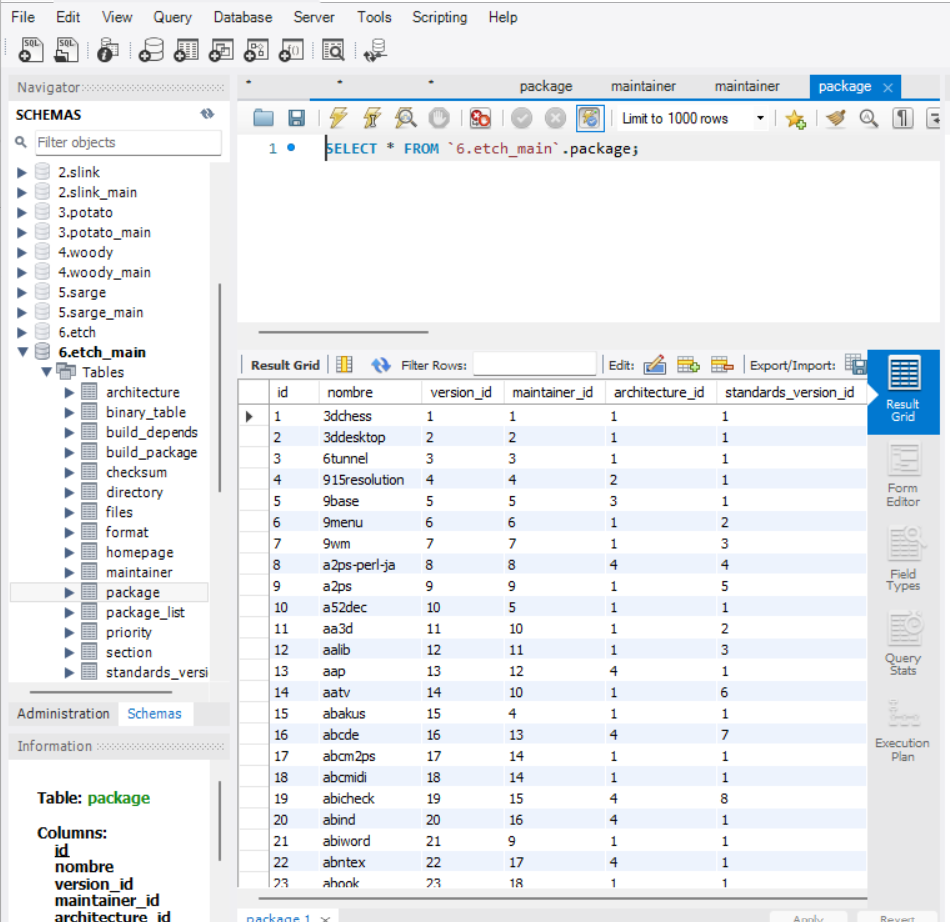
\includegraphics[width=10cm, keepaspectratio]{img/workbench.png}
	\caption{SQL Workbench. Fuente: elaboración propia.}
	\label{fig:workbench}
\end{figure}
%%%%%%%%%%%%%%%%%%%%%%%%%%%%%%%%%%%%%%%%%%%%%%%%%%%%%%%%%%%%%%%%%%%%%%%%%%%%%%%%
%%%%%%%%%%%%%%%%%%%%%%%%%%%%%%%%%%%%%%%%%%%%%%%%%%%%%%%%%%%%%%%%%%%%%%%%%%%%%%%%
% DISEÑO E IMPLEMENTACIÓN %
%%%%%%%%%%%%%%%%%%%%%%%%%%%%%%%%%%%%%%%%%%%%%%%%%%%%%%%%%%%%%%%%%%%%%%%%%%%%%%%%

\cleardoublepage
\chapter{Diseño e implementación}
\label{sec:diseno}

\section{Arquitectura general} 
\label{sec:arquitectura}
El objetivo de este proyecto es descubrir e investigar como evoluciona la distribución de Debian a lo largo de su historia y los factores que han cambiado o se han mantenido en releases posteriores junto con su explicación. Para ello hemos seguido estas fases:
\begin{figure}[h]
	\centering
	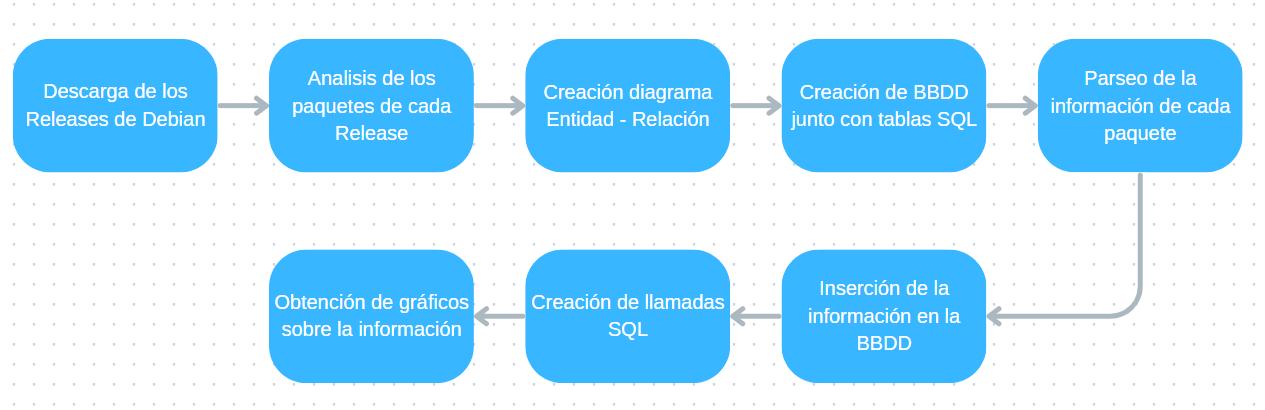
\includegraphics[width=14cm, keepaspectratio]{img/Diagrama_general.png}
	\caption{Fases del tratamiento de datos}
	\label{fig:Diagrama_general}
\end{figure}

Debemos analizar una gran cantidad de datos. Debian consta de 11 releases (lanzamientos) en los cuales se hallan un gran volumen de paquetes que va aumentando exponencialmente en releases posteriores.

Por ello, se necesita seguir una secuencia específica representada en la \textbf {Figura~\ref{fig:Diagrama_general}} para descargar, limpiar, ordenar y extraer estos datos de forma efectiva. 

Primero debemos descargar los diferentes releases de Debian desde su página oficial~\cite{debian:_releases}.
Con ello ya podremos analizar los diferentes paquetes que contienen y así poder diseñar el diagrama entidad - relación correspondiente.

Una vez tenemos el diseño completo, podremos comenzar con la creación de las diferentes BBDD (bases de datos) tal que cada release sea una base de datos con sus correspondientes tablas SQL.

En este punto creamos un script cuya funcionalidad será parsear los diferentes paquetes de cada release con el fin de extraer la información necesaria.

Una vez extraída dicha información creamos otro script que, conectándose a la BBDD correspondiente, introduzca los datos parseados en la BBDD para su posterior análisis.

Se crean una serie de Queries o llamadas SQL para poder obtener la información que necesitamos y así responder a los intereses del proyecto.

Por último, creamos una serie de gráficas y tablas para ayudar a la visualización de los resultados obtenidos en este estudio.


\section{Descarga de los releases de Debian} 
\label{sec:Descarga_de_los_releases_de_Debian}

Esta fase es la más rápida. 
\begin{figure}
	\centering
	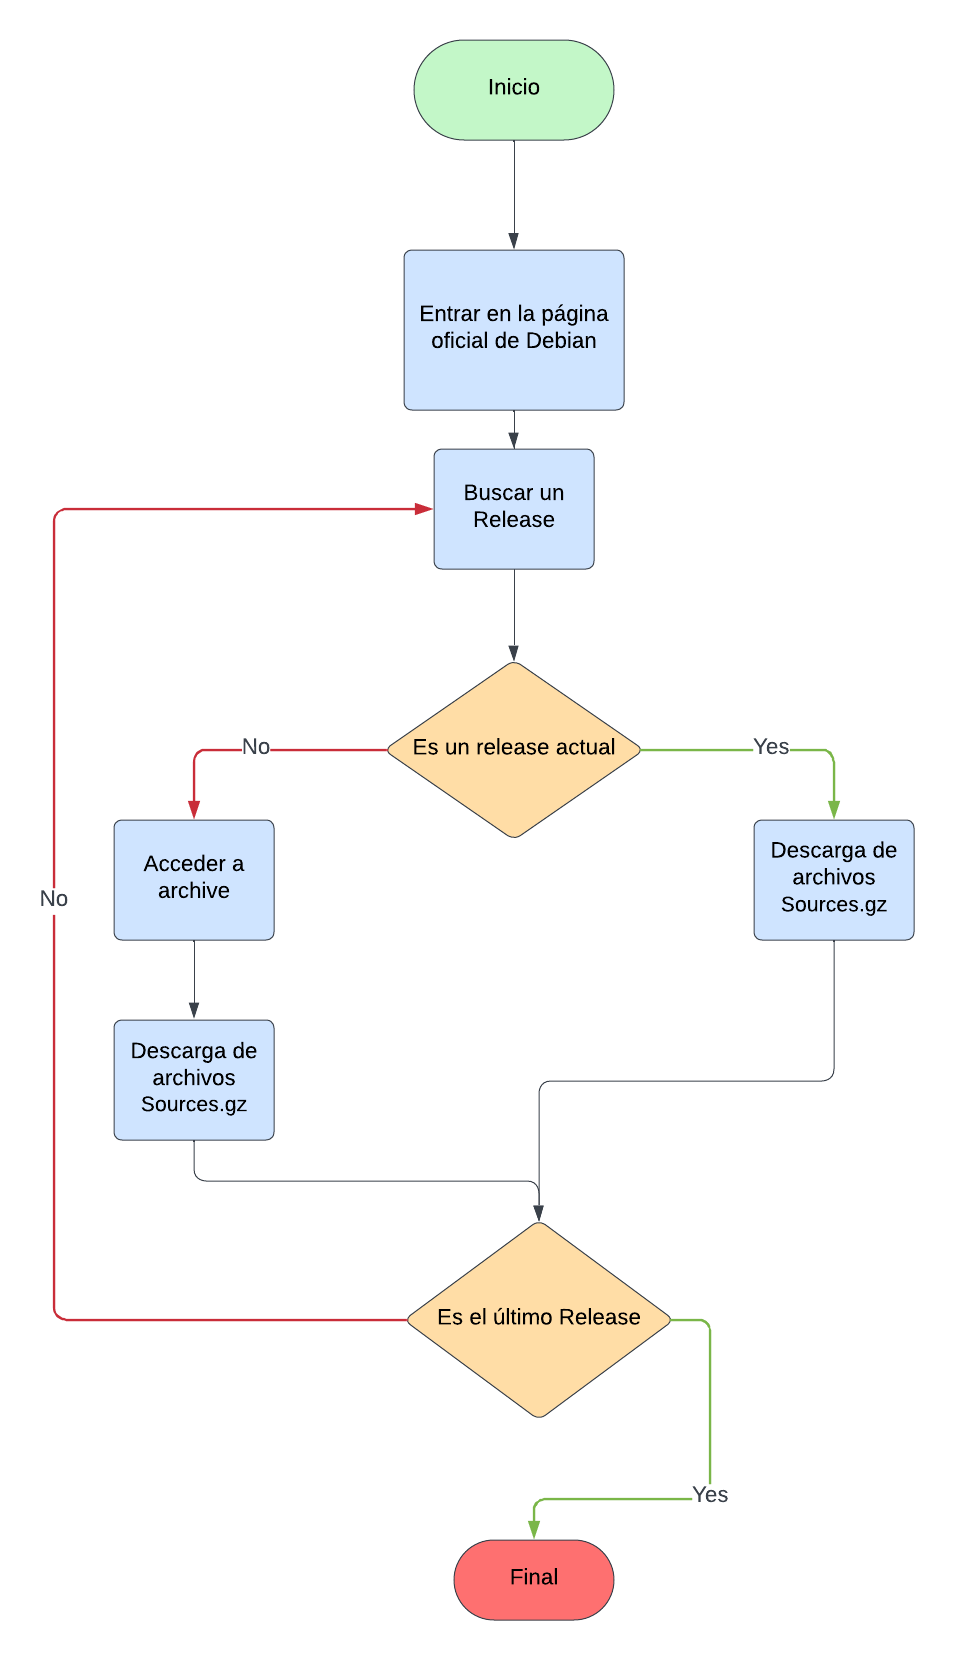
\includegraphics[width=10cm, keepaspectratio]{img/Descarga Releases.png}
	\caption{Diagrama de Flujo de la descarga de los Releases}
	\label{fig:flow_descarga}
\end{figure}
Conociendo las páginas donde encontrar los releases retirados~\cite{debian:_releases_archive} y los que siguen en uso~\cite{debian:_releases} (aportados por mi tutor Gregorio), podemos descargar sus diferentes archivos \textbf{main} en la \textbf{Figura~\ref{fig:Descarga_releases}} donde encontramos todos los paquetes de cada lanzamiento y con ello los datos que queremos tratar. Podemos ver el flujo en la \textbf{Figura~\ref{fig:flow_descarga}}.



\begin{figure}
	\centering
	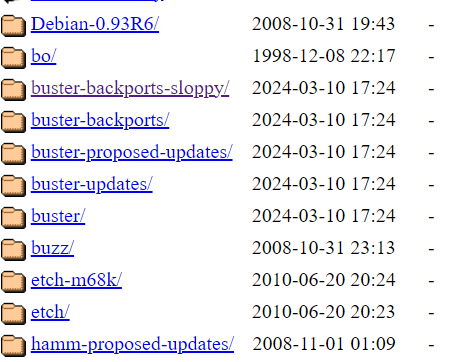
\includegraphics[width=10cm, keepaspectratio]{img/releases.png}
	\caption{Descarga de los datos de releases}
	\label{fig:Descarga_releases}
\end{figure}

\section{Análisis de los paquetes de cada release} 
\label{sec:analisis_de_los_paquetes}

En esta fase se requiere un estudio detallado de los diferentes atributos de cada paquete. Asignamos las entidades y las relaciones existentes entre los mismos para poder construir un diagrama valido para el diseño de las bases de datos posteriores.

Un paquete esta conformado por los atributos mostrados en la \textbf {Figura~\ref{fig:paquete}}.

\begin{figure}
	\centering
	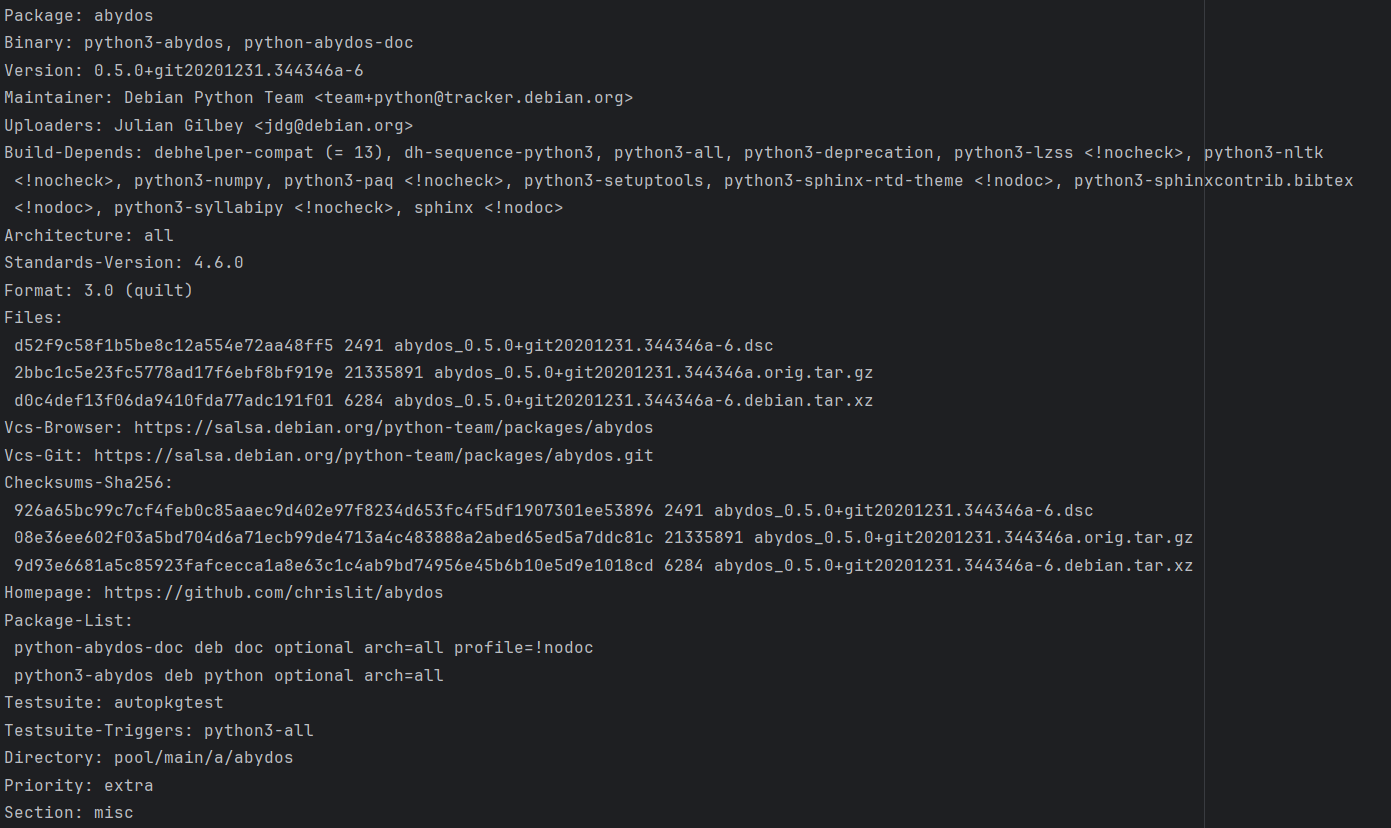
\includegraphics[width=15cm, keepaspectratio]{img/paquete.png}
	\caption{Atributos de un paquete.}
	\label{fig:paquete}
\end{figure}

\begin{figure}
	\centering
	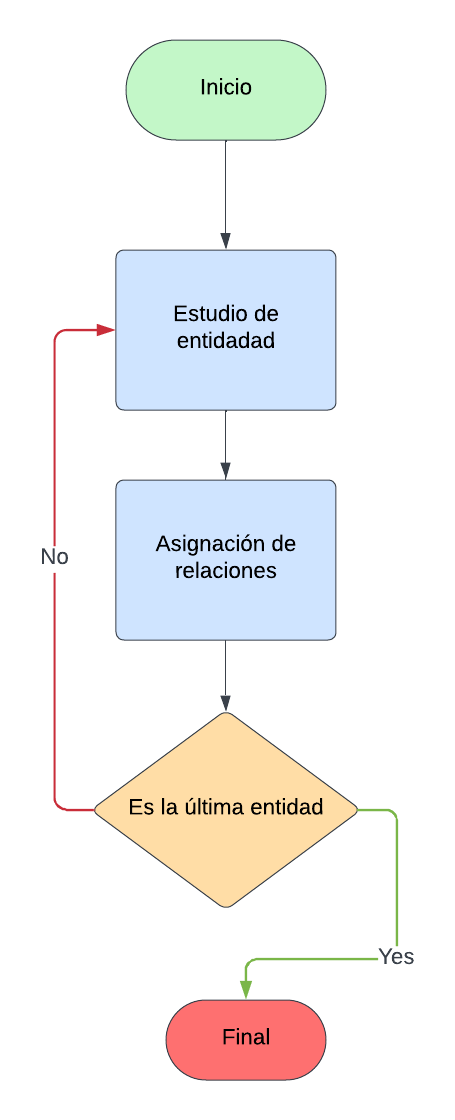
\includegraphics[width=9cm, keepaspectratio]{img/Estudio Atributos.png}
	\caption{Flujo del estudio de los atributos de un paquete}
	\label{fig:flujo_paquete}
\end{figure}

El siguiente proceso consta de la comparación de diferentes paquetes para entender que entidades hay y como relacionarlas:

\begin{itemize}
	\item \textbf {Package nombre}: siempre hay uno y es único. 
	\item \textbf {Binary}: mínimo hay uno o más. 
	\item \textbf {Version}: siempre hay uno y puede repetirse en varios paquetes.
	\item \textbf {Maintainer}: siempre hay uno y puede repetirse en varios paquetes. 
	\item \textbf {Uploaders}: mínimo hay uno o más y puede repetirse en varios paquetes. 
	\item \textbf {Build-Depends}: mínimo hay uno o más y puede repetirse en varios paquetes.  
	\item \textbf {Architecture}: siempre hay uno y puede repetirse en varios paquetes. 
	\item \textbf {Standards-Version}: siempre hay uno y puede repetirse en varios paquetes.
	\item \textbf {Format}: siempre hay uno y puede repetirse en varios paquetes. 
	\item \textbf {Files}:  mínimo hay uno o más y son únicos. 
	\item \textbf {Vcs-Browser}: (no está en todos los paquetes) máximo uno y es único. 
	\item \textbf {Vcs-Git}: (no está en todos los paquetes) máximo hay uno y es único. 
	\item \textbf {Checksums-Sha256}: mínimo hay uno o más y son únicos. 
	\item \textbf {Homepage}: (no está en todos los paquetes) máximo hay uno y puede repetirse en varios paquetes. 
	\item \textbf {Package-List}: mínimo hay uno o más y son únicos. 
	\item \textbf {Directory}: siempre hay uno y es único. 
	\item \textbf {Dgit}: (no está en todos los paquetes) máximo hay uno y es único. 
	\item \textbf {Testsuite}: (no está en todos los paquetes) máximo hay uno y puede repetirse en varios paquetes. 
	\item \textbf {Testsuite-Triggers}: (no está en todos los paquetes) puede haber uno o más y puede repetirse en varios paquetes. 
	\item \textbf {Priority}: siempre hay uno y puede repetirse en varios paquetes. 
	\item \textbf {Section}: siempre hay uno y puede repetirse en varios paquetes. 
\end{itemize}

Con esta información podemos comenzar con el diseño del diagrama.



\section{Creación diagrama Entidad - Relación} 
\label{sec:diagrama_entidad_relacion}
Un diagrama \textbf {entidad-relación}, también conocido como \textbf {modelo entidad relación o ERD~\cite{lucidchart:_diagramaERD}}, es un tipo de diagrama de flujo que ilustra cómo las entidades, como personas, objetos o conceptos, se relacionan entre sí dentro de un sistema.

\begin{figure}
	\centering
	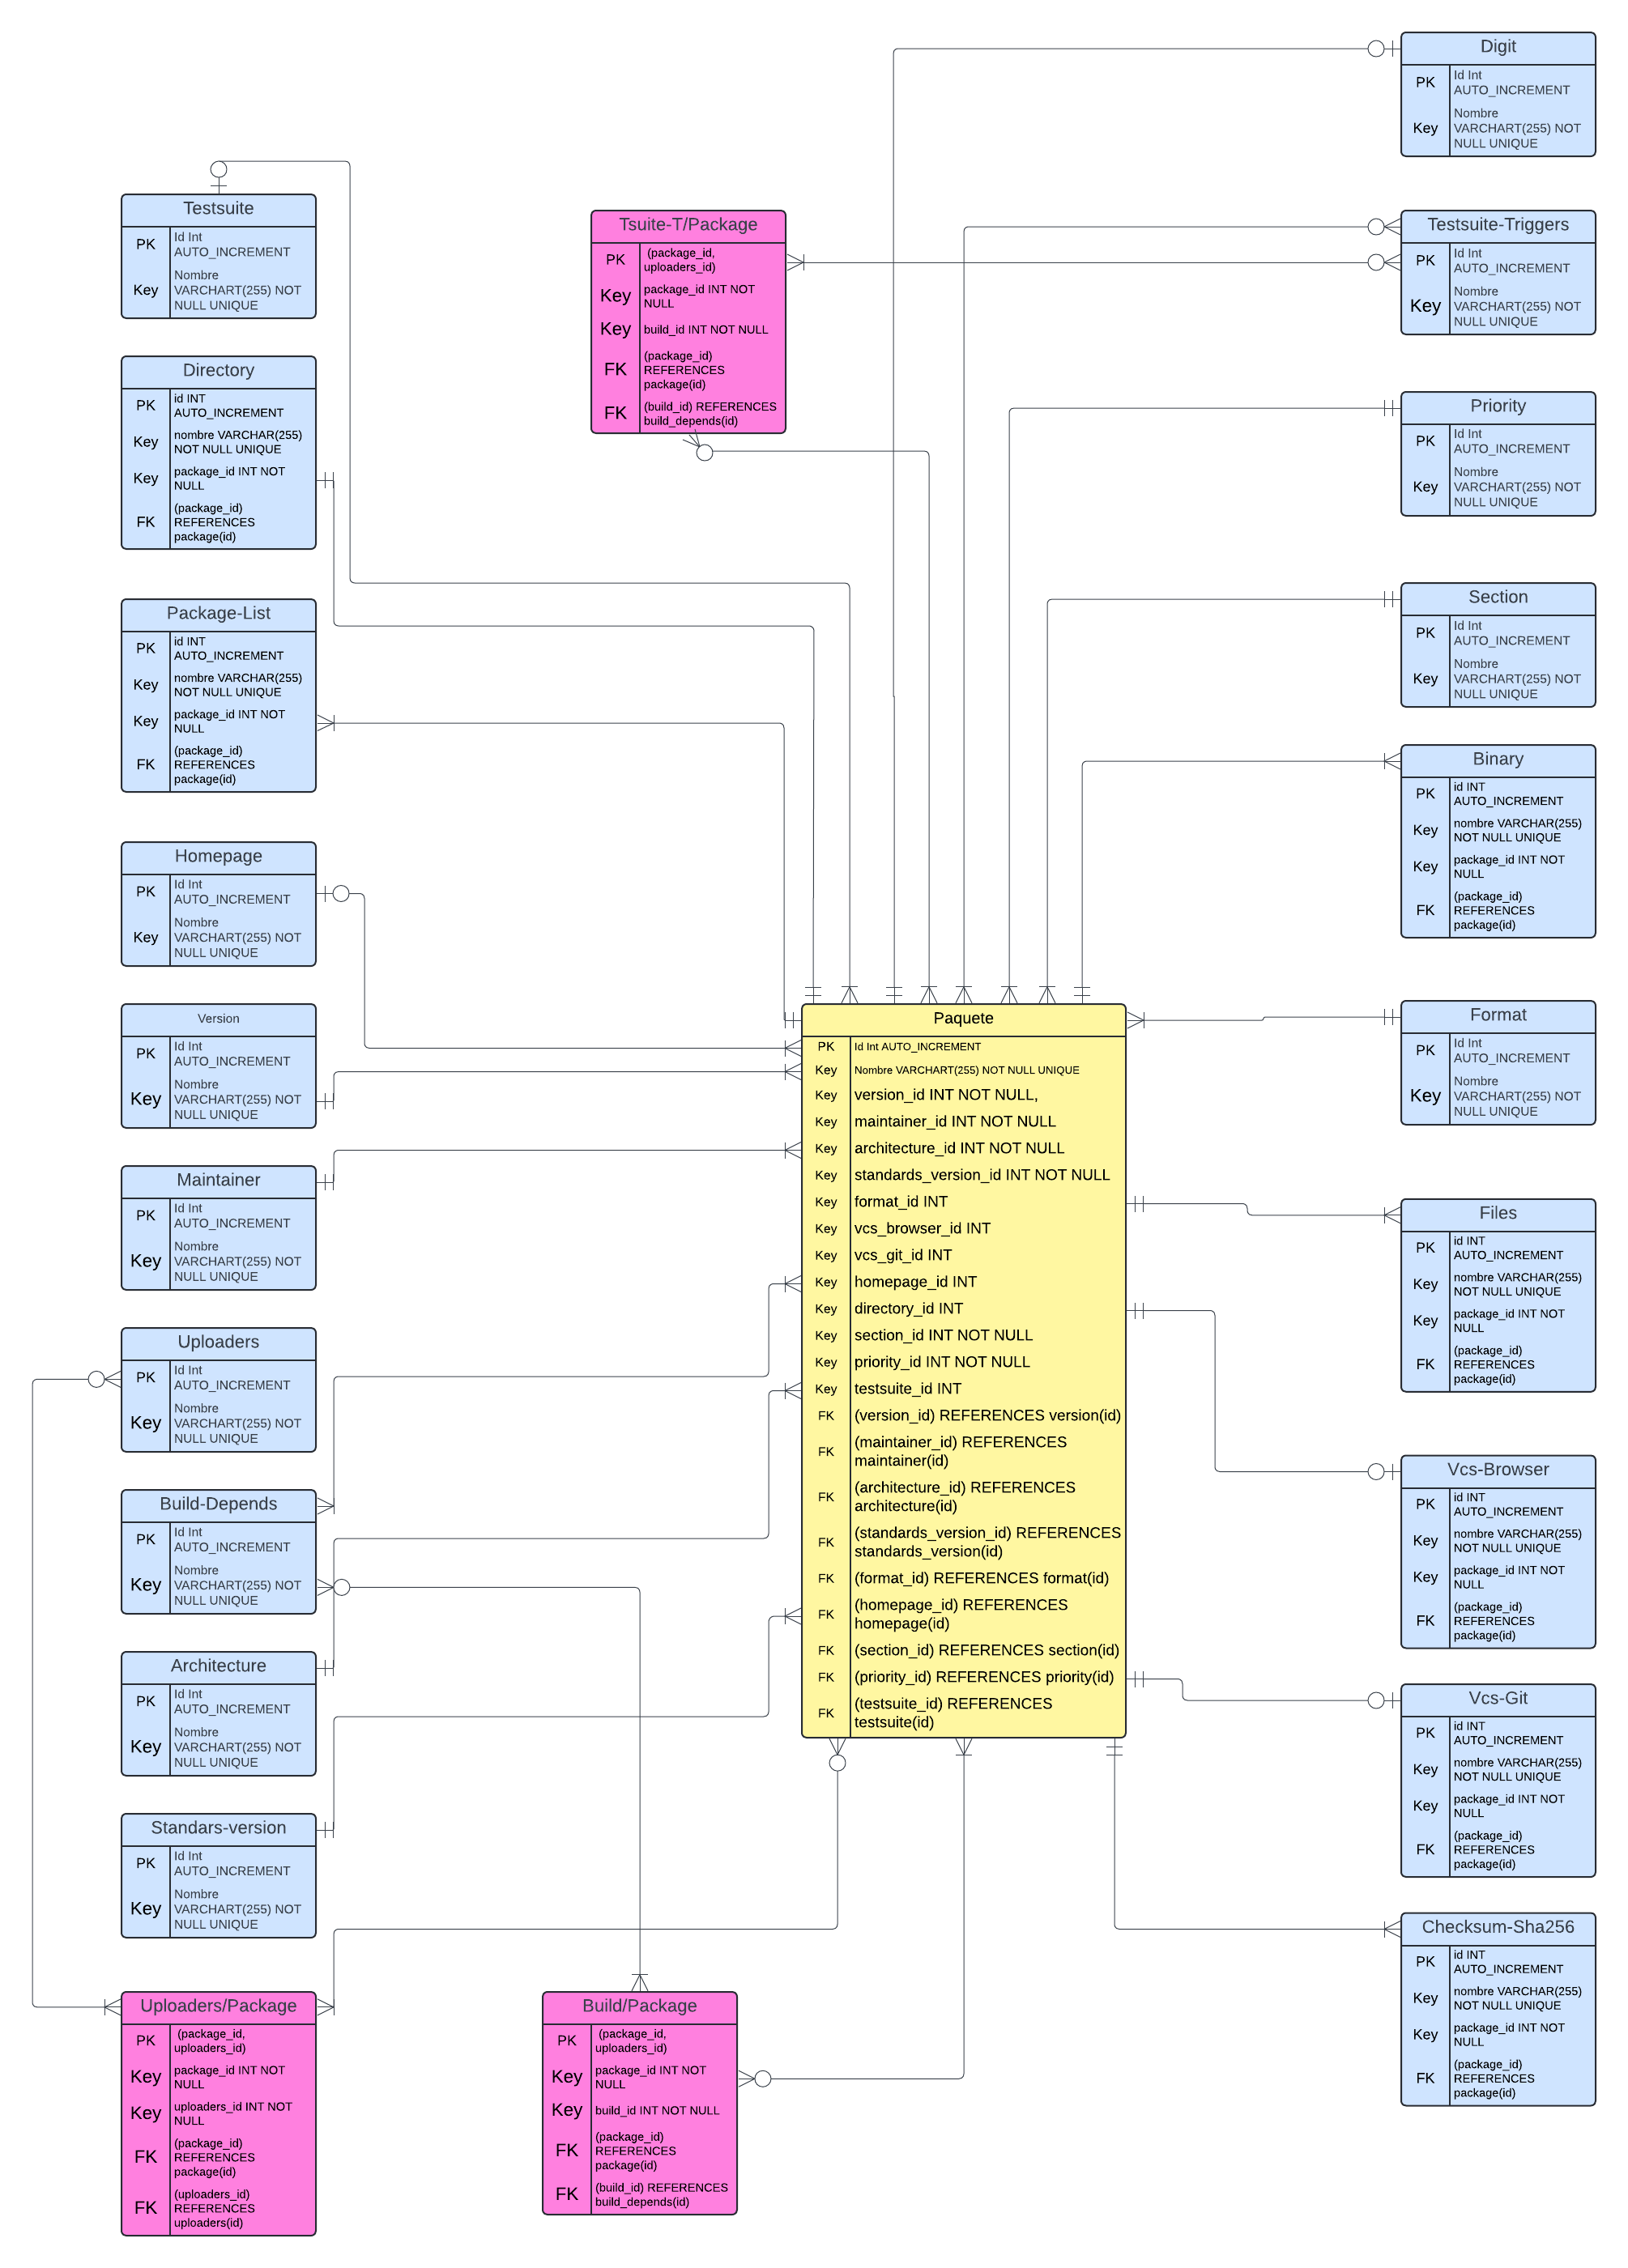
\includegraphics[width=17cm, keepaspectratio]{img/Diagrama_ER.png}
	\caption{Diagrama ER.}
	\label{fig:entidad_relación}
\end{figure}

\begin{figure}
	\centering
	\includegraphics[width=17cm, keepaspectratio]{img/leyenda_diagrama.png}
	\caption{Leyenda del Diagrama ER.}
	\label{fig:leyenda_diagrama}
\end{figure}

Los diagramas ER se usan a menudo para diseñar o depurar bases de datos relacionales en los campos de ingeniería de software, sistemas de información empresarial, educación e investigación. También emplean un conjunto definido de símbolos, tales como rectángulos, diamantes, óvalos y líneas de conexión para representar la interconexión de \textbf {entidades, relaciones y sus atributos.}

En la Figura~\ref{fig:entidad_relación} se observa el diseño del diagrama junto con la Figura~\ref{fig:leyenda_diagrama} que es su leyenda.

Cada rectángulo es una entidad que va unida a otras entidades mediante una serie de líneas que son los indicadores del tipo de relación que muestran.

En este caso todas las entidades tienen una relación de pertenencia debido a que un paquete contiene o no estas entidades.

En la \textbf {Figura~\ref{fig:leyenda_diagrama}} podemos ver el tipo de relación entre entidades:

\begin{enumerate}
\item Se muestra una relación de \textbf {1 a 1}, es decir, solo puede existir una entidad en el paquete obligatoriamente.

\item Se muestra una relación de \textbf {0 a 1}, es decir, pueden existir ninguna o una entidad en el paquete.

\item Se muestra una relación de \textbf {1 a infinito}, es decir, pueden existir una o muchas entidades en el paquete pero nunca puede no existir.

\item Se muestra una relación de \textbf {0 a infinito}, es decir, pueden existir ninguna, una o muchas entidades en el paquete.
\end{enumerate}

En este tipo de diagrama podemos observar como están diseñadas las tablas de la BBDD y como están relacionadas entre sí.

En la Figura\textbf {~\ref{fig:entidad_relación}} identificamos diferentes tablas:

\begin{itemize}
	\item \textbf {Tabla amarilla: }esta tabla es la principal ya que es \textbf {Package}. Tiene relaciones con todas las demás tablas. En ella podemos observar su \textbf {Primary Key} que es su \textbf {Id o identificador}, una serie de campos que son atributos (id's del resto de tablas) y sus \textbf {Foreing Key} que permiten poder relacionar las demás tablas con ella misma y así obtener valores correctos al realizar llamadas \textbf {SQL mediante Queries}.
	
	\item \textbf {Tablas azules: }estas tablas son las diferentes entidades que se encuentran en un paquete y están unidas a la tabla principal mediante las líneas, explicadas anteriormente, que muestran las relaciones que tienen.
	Cada una tiene su \textbf {Primary Key} que es su identificador, los atributos como el nombre y algunas contienen \textbf {Foreing Key} debido al tipo de relación entre tablas.
	
	\item \textbf {Tablas rosas: }estas son tablas intermedias que son necesarias para conectar tablas en las cuales no se puede insertar una \textbf {Foreing Key} en ninguna de las dos y por lo tanto no pueden relacionarse. Creando este tipo de tablas forzamos una conexión. Estas contienen una \textbf {Primary Key} especial conformada por los identificadores de ambas tablas y las \textbf {Foreing Key} asociadas a las tablas para poder relacionarlas.
	Son casos especiales en relaciones de \textbf {muchos a muchos}.
\end{itemize}

Una vez completadas las relaciones junto con las entidades se diseña la BBDD que va a acoger todos aquellos datos necesarios para el estudio.

\begin{figure}
	\centering
	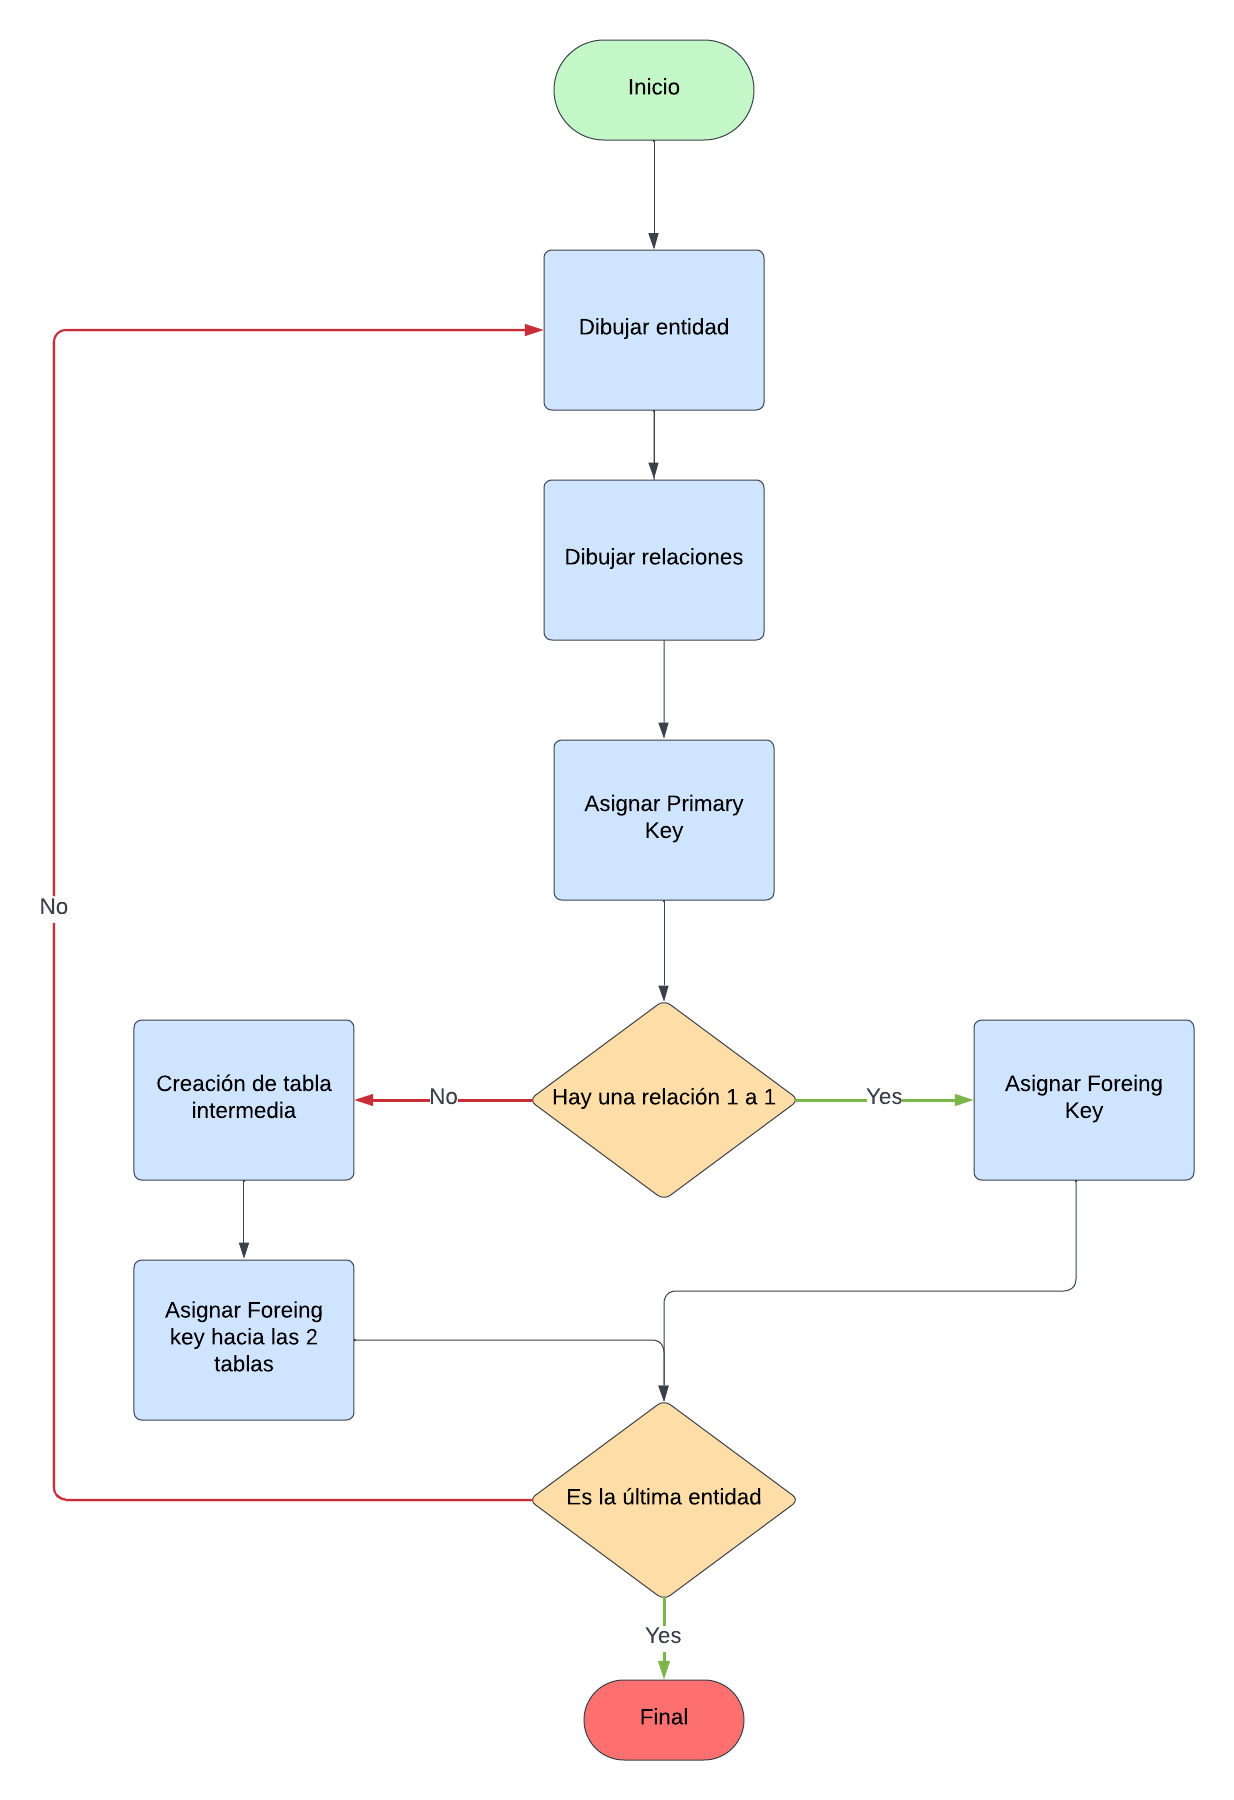
\includegraphics[width=15cm, keepaspectratio]{img/Creacion diagrama.png}
	\caption{Flujo de creación de diagrama Entidad - Relación}
	\label{fig:flujo creacion de diagrama}
\end{figure}

\section{Creación de BBDD junto con tablas SQL} 
\label{sec:creacion_BBDD}
En este punto se usan las aplicaciones MySQL Workbench y Pycharm.
\begin{figure}
	\centering
	\includegraphics[width=7cm, keepaspectratio]{img/Creación de tablas.png}
	\caption{Flujo de creación de BBDD}
	\label{fig:flujo creacion BBDD}
\end{figure}
Se crean las diferentes BBDD en MySQL para poder realizar la inserción de las tablas posteriormente como se muestra en la \textbf {Figura~\ref{fig:BBDDsql}}.

\begin{figure}
	\centering
	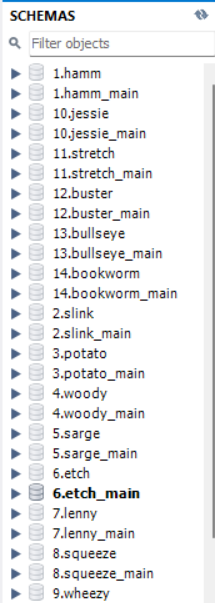
\includegraphics[width=4cm, keepaspectratio]{img/BBDDsql.png}
	\caption{Bases de datos}
	\label{fig:BBDDsql}
\end{figure}

El diseño de la BBDD depende directamente del diagrama realizado anteriormente. 
Este diagrama tiene una traducción a lenguaje SQL:
\begin{itemize}
	\item \textbf {Entidad 1 (uno y solo uno) Entidad 2}: cuando esto ocurre necesitamos crear una \textbf {foreing key} para relacionar las tablas de cada entidad. \textbf {Entidad 1} debe tener una foreign key para la \textbf {Entidad 2}.
	
	\begin{verbatim}
		"""
		CREATE TABLE IF NOT EXISTS package_list (
		id INT AUTO_INCREMENT PRIMARY KEY,
		nombre VARCHAR(255) NOT NULL UNIQUE,
		package_id INT NOT NULL,
		FOREIGN KEY (package_id) REFERENCES package(id)
		)
		"""
	\end{verbatim}
	
	Una \textbf {FOREIGN KEY}~\cite{thedataschool:_foreingkey} en SQL, es una clave (campo de una columna) que sirve para relacionar dos tablas. El campo FOREIGN KEY se relaciona o vincula con la PRIMARY KEY de otra tabla de la bbdd.
	
	La restricción \textbf {PRIMARY KEY}~\cite{thedataschool:_primarykey} SQL identifica de forma única cada registro en una tabla.
	Deben contener valores únicos y no pueden contener valores NULL.
	Una tabla solo puede tener una clave principal, que puede consistir en campos simples o múltiples.
	
	\item \textbf {{Entidad 1 (uno o muchos) Entidad 2}}: en este caso no tenemos claro que entidad debería acoger la foreign key por lo que se crea una tabla intermedia.
	Esta tabla constará de los identificadores de cada tabla como sus primary key.
	En ella es en la que se definirán las foreign key hacia ambas tablas y así poder relacionarlas.
	
	\begin{verbatim}
	"""
	CREATE TABLE IF NOT EXISTS uploaders_package (
	package_id INT NOT NULL,
	uploaders_id INT NOT NULL,
	PRIMARY KEY (package_id, uploaders_id),
	FOREIGN KEY (package_id) REFERENCES package(id),
	FOREIGN KEY (uploaders_id) REFERENCES uploaders(id)
	)
	"""
	\end{verbatim}
	
	Finalmente, se procede al desarrollo de un script que se conecte a la BBDD para crearlas y comenzar a usarlas.
	
	Para ello, debemos establecer una conexión con la BBDD indicando el host, puerto, usuario, contraseña y nombre de la BBDD.
	
	Todo se realiza a través de Python y con la librería mysql.connector.
	
	\begin{figure}
		\centering
		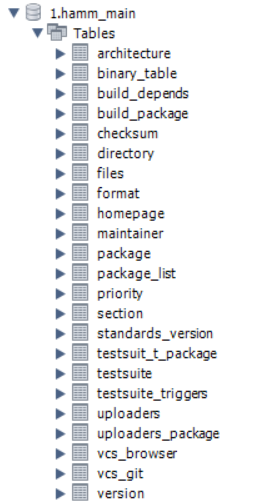
\includegraphics[width=6cm, keepaspectratio]{img/Tablas.png}
		\caption{Tablas BBDD}
		\label{fig:Tablas}
	\end{figure}
	
	

	
\end{itemize}

\section{Parseo de la información de los paquetes} 
\label{sec:parseo}
Tras la creación de las diferentes BBDD con sus tablas correspondientes, ahora debemos enfocarnos en obtener la información de interés para introducirla en dichas tablas SQL.

Para ello se diseña un script en Pycharm siguiendo estos pasos:

\begin{enumerate}
	\item \textbf{Lectura del archivo.} Las descargas de los releases realizadas en la sección~\ref{sec:Descarga_de_los_releases_de_Debian} las tratamos como ficheros de texto. Por ello debemos leer linea por linea todo el fichero e ir guardando la información relevante de cada paquete.
	
	\begin{verbatim}
		with open('Sources/14.Sources - bookworm-main.txt', 'r',
		 encoding='utf-8') as file:
		lines = iter(file.readlines())
	\end{verbatim}
	
	\item \textbf{Especificar qué datos son relevantes.} Se crea un array de strings con los diferentes nombres de los campos que queremos sacar para verificar si alguno se encuentra en la línea en la que estamos leyendo.
	
	\begin{verbatim}
		array_items = ['Package', 'Binary', 'Version', 'Maintainer',
		 'Uploaders', 'Build-Depends', 'Architecture',
		'Standards-Version', 'Format', 'Files', 'Vcs-Browser',
		 'Vcs-Git', 'Checksums-Sha256', 'Homepage',
		'Package-List', 'Directory', 'Priority', 'Section',
		 'Testsuite', 'Testsuite-Triggers']
	\end{verbatim}
	
	\item \textbf{Buscar los datos relevantes en el archivo.} Con el diseño del array ya podemos encontrar la información de interés. Recorremos línea a línea el archivo, comparamos si esa línea empieza con alguno de los items definidos seguido de \textbf{:} y parseamos la información guardándola en unas variables definidas anteriormente.
	
	\begin{verbatim}
		for line in lines:
		field, *value = map(str.strip, line.split(': ', 1))
		value = value[0] if value else ''
		
		if field in array_items:
	
			if field == "Package":
				package = value
			
			elif field == "Binary":
				binary = value
			...
	\end{verbatim}
	
		\item \textbf{Identificar el final del paquete.} En un archivo hay miles de paquetes juntos separados por una línea en blanco. Este será nuestro identificador de que hemos recogido la información de un paquete. Si encuentra dicha línea, se llama a la función que nos permitirá insertar esta información en las diferentes tablas.
		
	\begin{verbatim}
		 elif not line.strip():
		# Esto indica el final de la información del paquete
			insertar_info(package, binary, version, maintainer,
			 uploaders, build_depends, architecture,
			standards_version, format1, files_list, vcs_browser,
			 vcs_git, check_list, homepage,
			package_list, directory, priority, section, testsuite,
			 testsuite_triggers)
	\end{verbatim}
	
		\item \textbf{Restaurar las variables.} Este proceso es iterativo debido a que se realiza para cada paquete dentro de cada release. Necesitamos vaciar las variables para volver a obtener los datos de los próximos paquetes.
		
\end{enumerate}

\section{Inserción de la información en la BBDD}
\label{sec:insercion_BBDD}
Una vez parseada la información de un paquete, debemos realizar la inserción en la BBDD. Esto se ejecuta mediante otro script en Pycharm y con la librería mysql.connector.

\begin{figure}
	\centering
	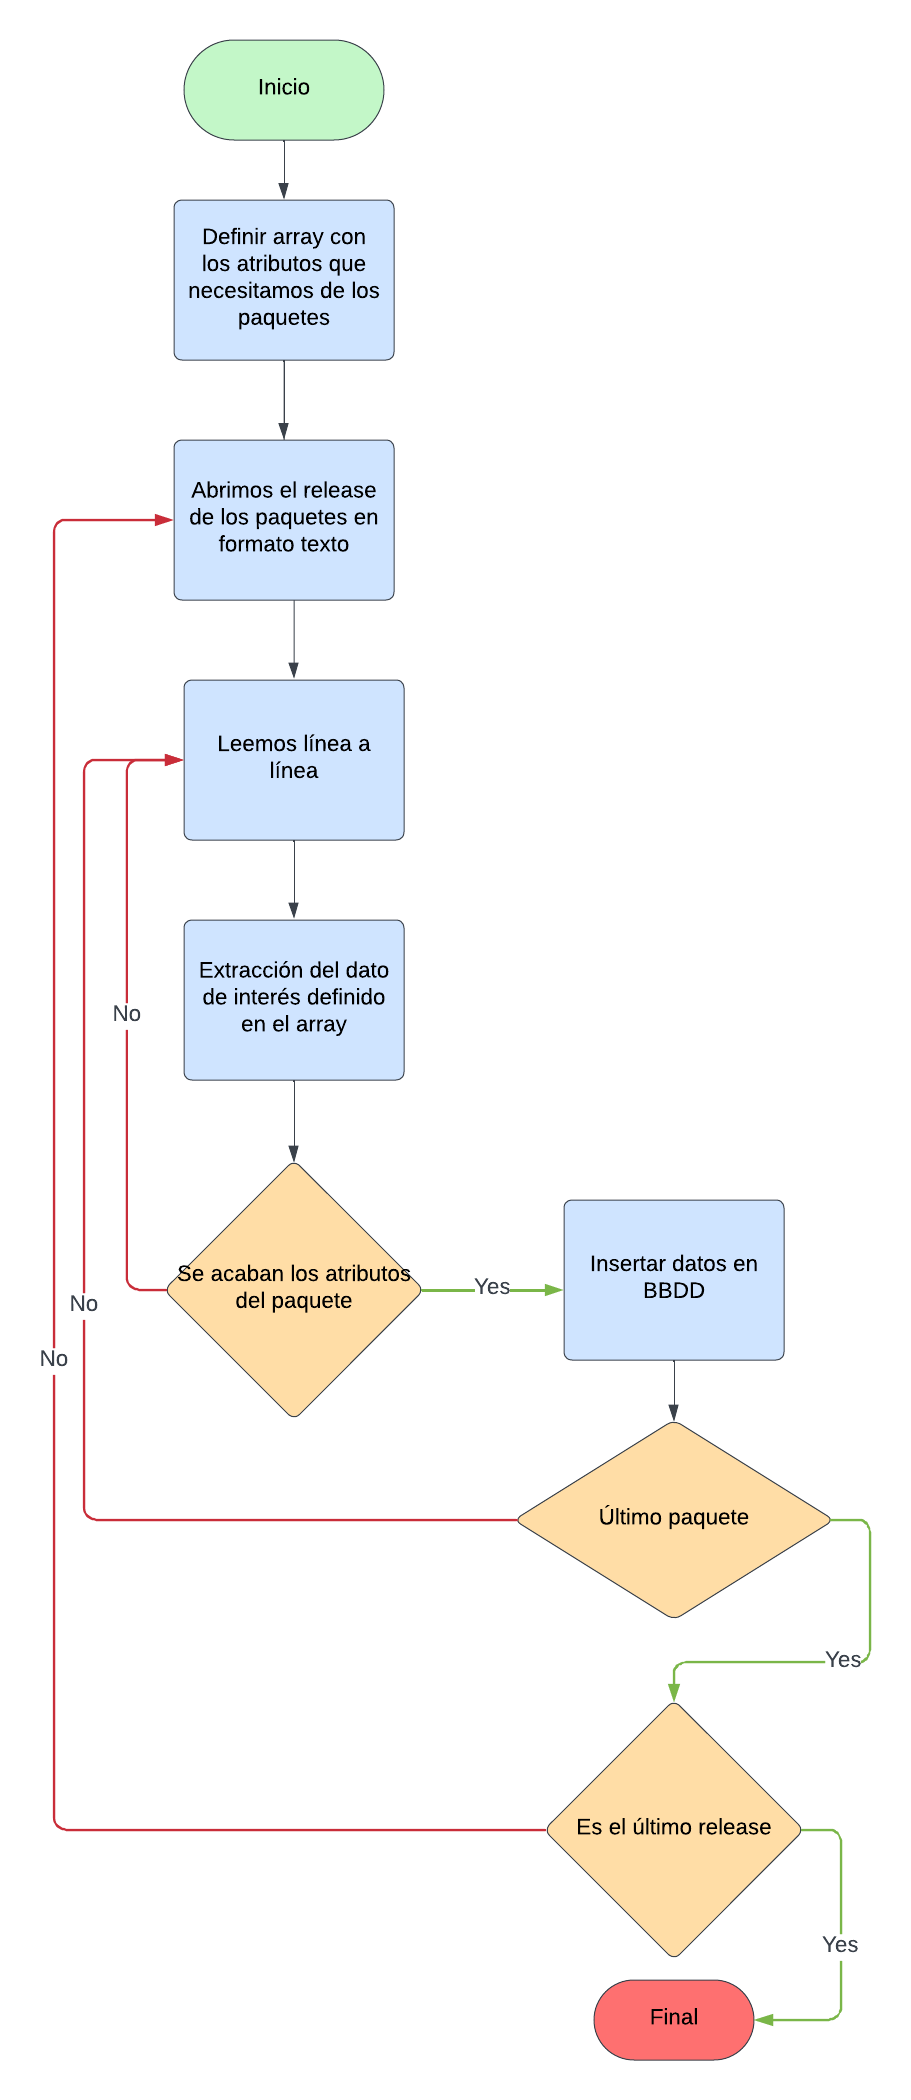
\includegraphics[width=10cm, keepaspectratio]{img/Insertar BBDD.png}
	\caption{Flujo de inserción de los datos en BBDD}
	\label{fig:flujo insertar datos}
\end{figure}


\begin{enumerate}
		\item \textbf{Conexión a la BBDD.} Primero debemos conectarnos a la BBDD para obtener la funcionalidad de insertar en ella. Debemos introducir los siguientes datos:
		\begin{verbatim}
			conexion = mysql.connector.connect(
			host='localhost',
			port=3306,
			user='root',
			password='xxxx',
			db='14.bookworm_main'
		)
		\end{verbatim} 
		
		\item \textbf{Creación de diccionario.} Necesitamos asociar los diferentes valores, de las variables de la sección~\ref{sec:parseo}, a los nombres de las tablas para facilitar la lógica de dicho script.
		\begin{verbatim}
			datos = {
				"version": version,
				"maintainer": maintainer,
				"uploaders": uploaders,
				"build_depends": build_depends,
				"architecture": architecture,
				"standards_version": standards_version,
				"format": format1,
				"section": section,
				"priority": priority,
				...
		\end{verbatim} 
		
		\item \textbf{Inserción de los datos.} Finalmente pasamos a el objetivo final de este punto, la inserción. Tenemos varios casos que deben ser contemplados para su óptima realización:
		
		\begin{itemize}
			\item \textbf{Valores vacíos:} en este caso debemos comprobar si la variable en cuestión tiene un valor predeterminado o viene vacío. Hay paquetes en los que no existen ciertas entidades como vimos en la sección~\ref{sec:analisis_de_los_paquetes}. Se actualiza el valor a None para evitar fallos en la BBDD al insertar.
			
			\item \textbf{Datos duplicados: } hay entidades que se repiten en múltiples paquetes como las versiones o los maintainer. Debemos tener en cuenta que, al crear las tablas, se ponen restricciones como los identificadores únicos. Esto significa que no se pueden meter duplicados y por ello debemos tenerlo en cuenta. Para ello, buscamos si el valor ya se encuentra en la tabla, si se confirma, se ignora para evitar errores en las tablas SQL.
			
			\item \textbf{Valores múltiples: } hay entidades que tienen varios datos separados por comas como Build-Depends. En estos casos debemos separarlo por comas creando un array. Después, se recorre el array y se va metiendo uno a uno verificando que no sean duplicados.
			
			\begin{figure}[h]
				\centering
				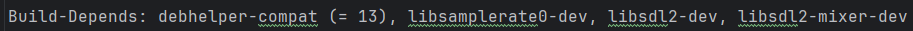
\includegraphics[width=15cm, keepaspectratio]{img/Build_depends.png}
				\caption{Build Depends}
				\label{fig:Build_depends}
			\end{figure}
			
			\item \textbf{Files o Checksums-Sha256: } son 2 casos en los que no tenemos comas y vienen varios datos por entidad. Cuando verifiquemos que una linea del paquete empieza por estos 2 casos debemos cambiar la lógica. Saltamos a las siguientes lineas guardando todos los datos en un array. Posteriormente se recorrerá y se insertarán en las diferentes tablas.
			
			\begin{figure}[h]
				\centering
				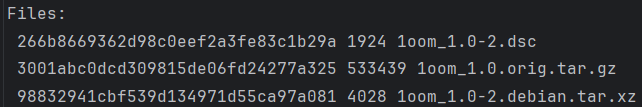
\includegraphics[width=15cm, keepaspectratio]{img/Files.png}
				\caption{Atributo Files de cada paquete en el que se muestran diferentes archivos contenidos en él.}
				\label{fig:Files}
			\end{figure}
		\end{itemize}
		
		Por último, hay que vincular diferentes tablas a través de sus foreign keys.
		
		Al insertar un paquete, guardamos su id. De esta forma, al insertar otra entidad diferente (en otra tabla) sabemos que id de paquete tiene y con ello podemos referenciarlo sin problemas.
		
		Esto es de suma importancia debido al diseño de las posteriores Queries.
\end{enumerate}

\section{Creación de Queries SQL}
\label{sec:queries}

Para este proceso se necesita de nuevo un script en Pycharm que se conecte a la BBDD y, a través de lenguaje SQL, realice llamadas especificas a la misma. De esta forma obtendremos la información que se necesita.

\begin{figure}
	\centering
	\includegraphics[width=6cm, keepaspectratio]{img/Creación queries.png}
	\caption{Flujo de creación de queries}
	\label{fig:flujo creacion queries}
\end{figure}

\begin{enumerate}
	\item \textbf{Conexión a la BBDD.} Primero debemos conectarnos a la BBDD para obtener la funcionalidad de realizar llamadas sobre ella como en la sección~\ref{sec:insercion_BBDD}.
	
	\item \textbf{Lenguaje de manipulación de datos~\cite{geotalleres:_sql}.} Proporcionado por el sistema de gestión de base de datos, permite a los usuarios llevar a cabo las tareas de consulta o manipulación de los datos, organizados por el modelo de datos adecuado. 

	\begin{itemize}
		\item \textbf{Comandos}: para insertar como en la sección~\ref{sec:insercion_BBDD}, actualizar o borrar pero en este caso se quiere consultar por lo que usaremos `SELECT'.
		
		\item \textbf{Clausulas}: son condiciones de modificación utilizadas para definir los datos que desea seleccionar o manipular. En nuestro caso usaremos `WHERE'.
		
		\item \textbf{Operadores Lógicos}: como \textbf{AND, OR y NOT}.
		
		\item \textbf{Operadores de comparación}: como \textbf{LIKE, IN, BETWEEN, etc.}
		
	\end{itemize}
	
	\item \textbf{Queries.} Se crean diferentes funciones para separar las llamadas y facilitar la comprensión del código. 
	
	
	
	Este sería un ejemplo de una Query que devuelve el numero de maintainers total que hay en cada release o BBDD:
	
	\begin{verbatim}
		...
		consulta = "SELECT COUNT(*) FROM maintainer"
		cursor.execute(consulta)
		...
	\end{verbatim} 
	
	Cuenta el número de mantenedores que hay en la tabla `maintainer' de la base de datos actual. Esta consulta va dentro de un bucle que hace el cálculo para todas las BBDD.
	
	Cada llamada contesta a las preguntas realizadas para este estudio obteniendo de forma eficiente la información de las BBDD.
	 
\end{enumerate}

\section{Obtención de gráficas informativas}
\label{sec:graficas}

En este apartado sigue siendo necesario la creación de un script en Pycharm pero con la librería `Matplotlib'.

Con el diseño de las queries del apartado~\ref{sec:queries} obtenemos la información necesaria para responder a las diferentes cuestiones planteadas en este estudio.
Para ayudar a la comprensión de estos datos debemos crear diferentes gráficas.
Visualizar los resultados facilita la interpretación de los mismos para obtener unas conclusiones óptimas.

Para ello es necesario:
\begin{enumerate}
	\item \textbf{Queries del script anterior}: como explicamos anteriormente, vamos a realizar una representación visual de la información obtenida por las queries por lo que son imprescindibles.
	
	\begin{verbatim}
		resultados_paquetes = obtener_numero_paquetes(array_database1)
	\end{verbatim} 
	
	\item \textbf{Definir los ejes}: estas gráficas aportarán información del número de paquetes existentes y el número de mantenedores que trabajan con cada versión. Debemos definir cada eje con sus correspondientes etiquetas para evitar confusiones.
	
	\begin{verbatim}
		x = ["Julio1998", "Marzo1999", "Agosto2000", "Julio2002",
		 "Junio2005", "Abril2007", "Febrero2009", "Mayo2014",
		  "Junio2016", "Junio2018", "Junio2020", "Septiembre2022",
		   "Febrero2024"]
	\end{verbatim} 
	
	\begin{itemize}
		\item \textbf{Eje x}: fechas de los lanzamientos de los diferentes releases.
		
		\item \textbf{Eje y}: número de paquetes o mantenedores (dependiendo de la gráfica) que hay en cada release.
	\end{itemize}
	
	\item \textbf{Conversión del eje x a objeto fecha}: este es uno de los detalles más importantes para presenciar y entender de forma correcta la información. Se trata de convertir cada etiqueta del eje x como `Junio2022' a un objeto temporal. De esta forma se representará un espacio mayor o menor en el eje x dependiendo de la distancia entre fechas de lanzamiento de los releases.
	
	
	\item \textbf{Creación del gráfico}: en nuestro caso será un gráfico de barras. Para ello definimos el tipo de gráfica que queremos, agregamos los datos obtenidos por las queries, configuramos los diferentes ejes junto con el título de la gráfica y la mostramos.
\end{enumerate}

\begin{figure}
	\centering
	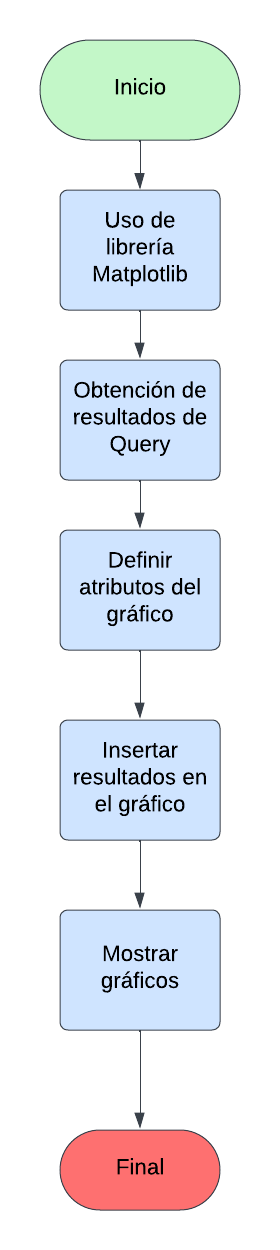
\includegraphics[width=5cm, keepaspectratio]{img/Creación gráficas.png}
	\caption{Flujo de creación de gráficas}
	\label{fig:flujo creacion graficas}
\end{figure}


%%%%%%%%%%%%%%%%%%%%%%%%%%%%%%%%%%%%%%%%%%%%%%%%%%%%%%%%%%%%%%%%%%%%%%%%%%%%%%%%
%%%%%%%%%%%%%%%%%%%%%%%%%%%%%%%%%%%%%%%%%%%%%%%%%%%%%%%%%%%%%%%%%%%%%%%%%%%%%%%%
% RESULTADOS %
%%%%%%%%%%%%%%%%%%%%%%%%%%%%%%%%%%%%%%%%%%%%%%%%%%%%%%%%%%%%%%%%%%%%%%%%%%%%%%%%

\cleardoublepage
\chapter{Resultados}
\label{chap:resultados}

En este capítulo se muestran los diferentes resultados a las preguntas que nos realizamos en este proyecto. De esta forma podremos observar la información obtenida y sacar conclusiones a partir de ella.

\section{¿Cuántos mantenedores tiene Debian y cómo cambia este número con el tiempo?}
\label{sec:pregunta_1}
Esta distribución lanza nuevas versiones cada cierto tiempo como mostramos en la sección~\ref{subsec:proyecto debian}. Cada versión está formada por múltiples paquetes y cada paquete lo mantiene una persona (aunque puede mantener varios paquetes a la vez). El número de mantenedores de dichos paquetes no es fijo ya que en cada versión pueden incorporarse nuevos o, por el contrario, abandonarlo.

Y por ello nos preguntamos,  \textbf{¿cual es el número de mantenedores en cada versión?} Y si no es fijo, \textbf{¿aumenta o disminuye en versiones posteriores?}

Para responderla se han aplicado unas queries con las que se obtiene el número total de maintainers únicos en cada versión/release.

Una vez ejecutadas las queries se obtienen estos resultados:

\begin{table}[h]
	\begin{center}
		\begin{tabular}{|l|l|r|} % Cambiado l por r en la última columna
			\hline
			Fecha           & Release  & Maintainers \\ \hline
			Julio 1998      & Hamm     & 255         \\ \hline
			Marzo 1999      & Slink    & 362         \\ \hline
			Agosto 2000     & Potato   & 530         \\ \hline
			Julio 2002      & Woody    & 986         \\ \hline
			Junio 2005      & Sarge    & 1.490       \\ \hline
			Abril 2007      & Etch     & 1.760       \\ \hline
			Febrero 2009    & Lenny    & 1.971       \\ \hline
			Mayo 2014       & Squeeze  & 2.173       \\ \hline
			Junio 2016      & Wheezy   & 2.286       \\ \hline
			Junio 2018      & Jessie   & 2.468       \\ \hline
			Junio 2020      & Stretch  & 2.412       \\ \hline
			Septiembre 2022 & Buster   & 2.413       \\ \hline
			Febrero 2024    & Bullseye & 2.293       \\ \hline
		\end{tabular}
		\caption{Tabla de versiones de Debian}
	\end{center}
\end{table}



Una vez obtenidos los resultados podemos mostrar las gráficas para visualizarlos.
\begin{figure}
	\centering
	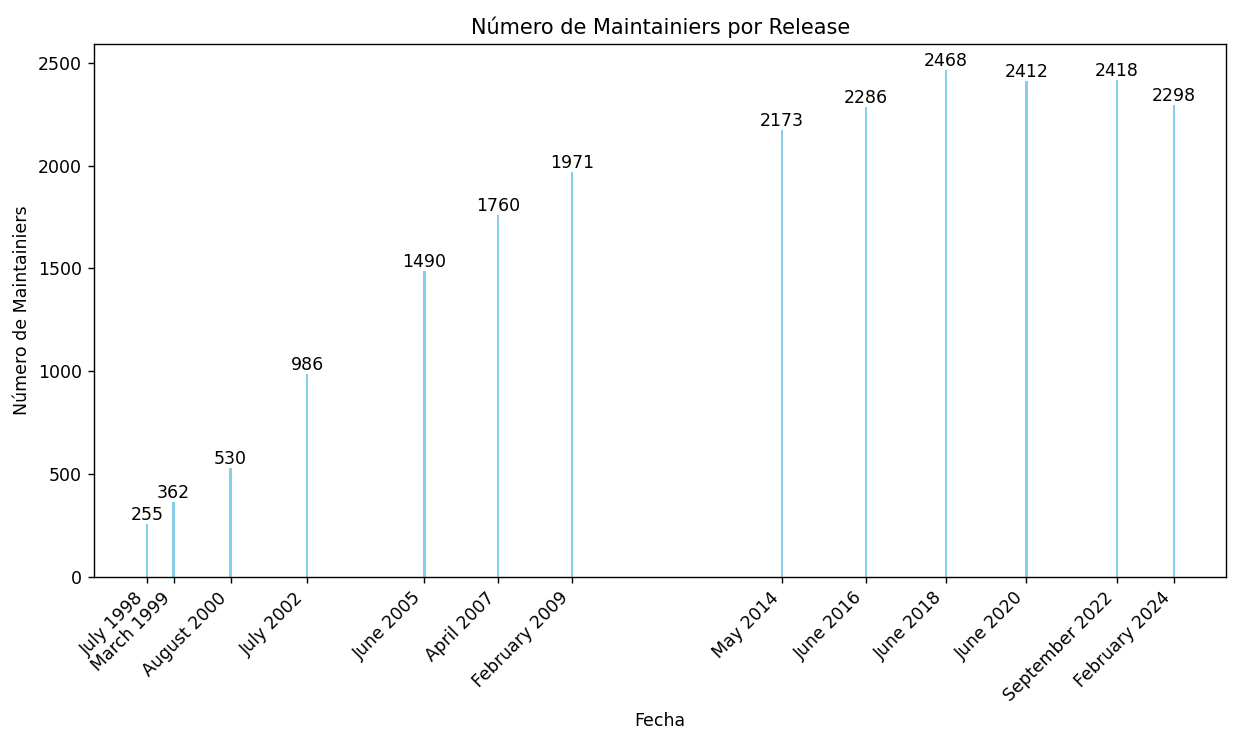
\includegraphics[width=15cm, keepaspectratio]{img/Figura2_buena_maintainers.png}
	\caption{Número de maintainers de cada release}
	\label{fig:mantenedores}
\end{figure}


En la  \textbf{Figura~\ref{fig:mantenedores}} se observa el número de mantenedores totales y únicos de por cada release. 
Gracias a que el eje x es un objeto temporal, podemos apreciar la diferencia entre tiempos de lanzamiento sobre cada release.
	\begin{itemize}
	\item  Se encuentran dos parones en los lanzamientos de los release entre julio de 2002 y junio de 2005, y entre febrero de 2009 y mayo de 2014 (alargándose más en el tiempo que el anterior).
	
	\item También podemos ver la tendencia que sigue la gráfica con respecto a los maintainers. Hasta Junio de 2018 hay una subida del número de maintainers pero a partir de este release se aprecia una pequeña bajada de los mismos.
\end{itemize}

También se ha calculado el número de paquetes que encontramos en cada release mediante una query y podemos ver el resultado en la \textbf{Figura~\ref{fig:paquetes}}.

\begin{figure}
	\centering
	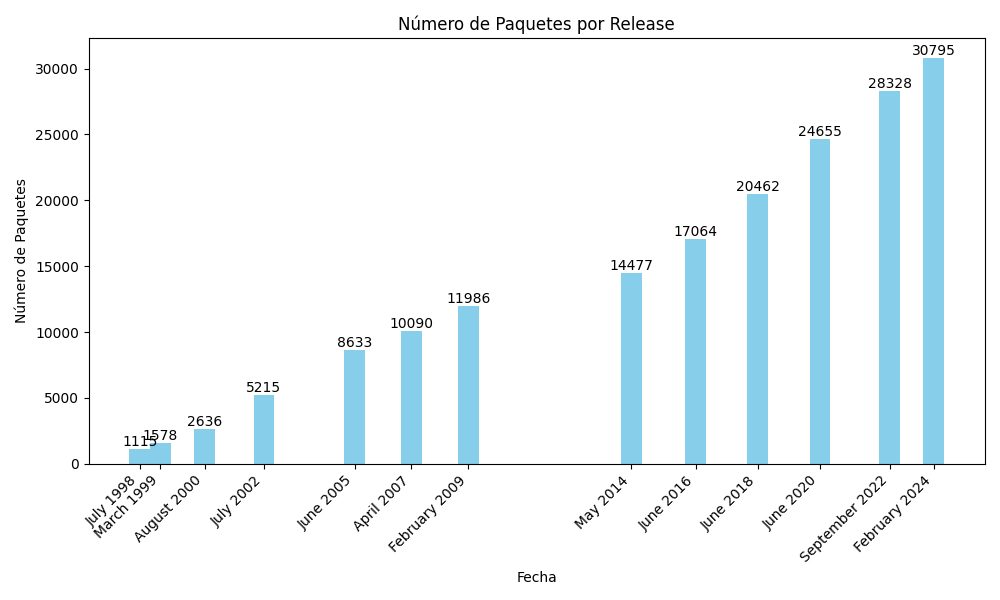
\includegraphics[width=15cm, keepaspectratio]{img/paquetes_releases.png}
	\caption{Número de paquetes de cada release}
	\label{fig:paquetes}
\end{figure}

Como se puede apreciar, hay un aumento exponencial en la cantidad de paquetes llegando hasta los 30.795 en la última versión.

\section{¿Existe una tendencia hacia la formación de equipos de mantenedores?}
\label{sec:pregunta_2}
La distribución Debian estaba conformada en sus orígenes por una serie de personas que trabajaban para su desarrollo. Con el paso del tiempo comenzaron con la agrupación de estos para la creación de grupos Debian. Con ello se organizarían mejor y podrían desempeñar un óptimo trabajo especializándose en un área concreta.


Por ello nos preguntamos si existiera dicha tendencia a la creación de equipos y como varía con el tiempo.

Podemos diferenciar que maintainers son equipos o personas individuales debido al `nombre' del campo `maintainer' de cada paquete. Estos nombres suelen contener la palabra \textbf{Team} o \textbf{Group} como vemos en las \textbf{Figuras~\ref{fig:ejemplo_equipo_1} y~\ref{fig:mantenedores}}

\begin{figure}
	\centering
	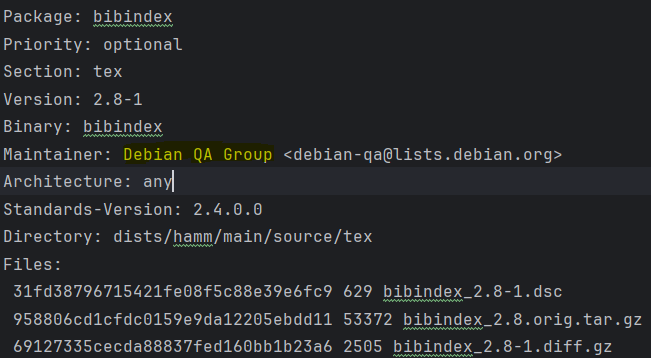
\includegraphics[width=15cm, keepaspectratio]{img/Ejemplo equipo 1.png}
	\caption{Ejemplo de nombre de equipo de maintainers}
	\label{fig:ejemplo_equipo_1}
\end{figure}

\begin{figure}
	\centering
	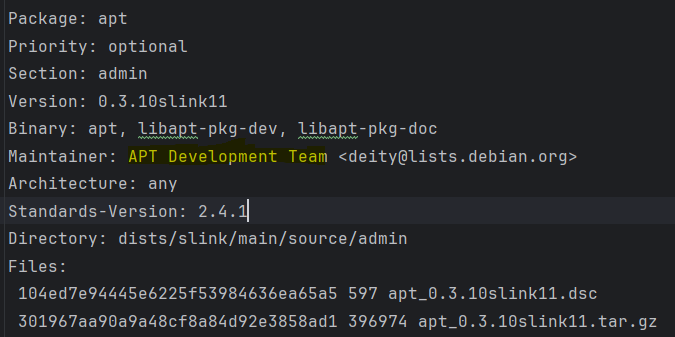
\includegraphics[width=15cm, keepaspectratio]{img/Ejemplo equipo 2.png}
	\caption{Ejemplo de nombre de equipo de maintainers}
	\label{fig:ejemplo_equipo_2}
\end{figure}

Para ello lanzamos la query para obtener el número de equipos en cada release.

Una vez ejecutado estos son los resultados:

\begin{table}[h]
	\begin{center}
		\begin{tabular}{|l|l|r|}
			\hline
			Fecha         & Release  & Equipos \\ \hline
			Julio 1998     & Hamm     & 1       \\ \hline
			Marzo 1999     & Slink    & 2       \\ \hline
			Agosto 2000    & Potato   & 8       \\ \hline
			Julio 2002     & Woody    & 8       \\ \hline
			Junio 2005     & Sarge    & 31      \\ \hline
			Abril 2007     & Etch     & 79      \\ \hline
			Febrero 2009   & Lenny    & 118     \\ \hline
			Mayo 2014      & Squeeze  & 147     \\ \hline
			Junio 2016     & Wheezy   & 168     \\ \hline
			Junio 2018     & Jessie   & 196     \\ \hline
			Junio 2020     & Stretch  & 210     \\ \hline
			Septiembre 2022 & Buster   & 289     \\ \hline
			Febrero 2024   & Bullseye & 317     \\ \hline
		\end{tabular}
	\end{center}
	\caption{Tabla de versiones de Debian con equipos}
\end{table}


Obteniendo los datos analíticamente, mostramos la gráfica para visualizar la información.

\begin{figure}
	\centering
	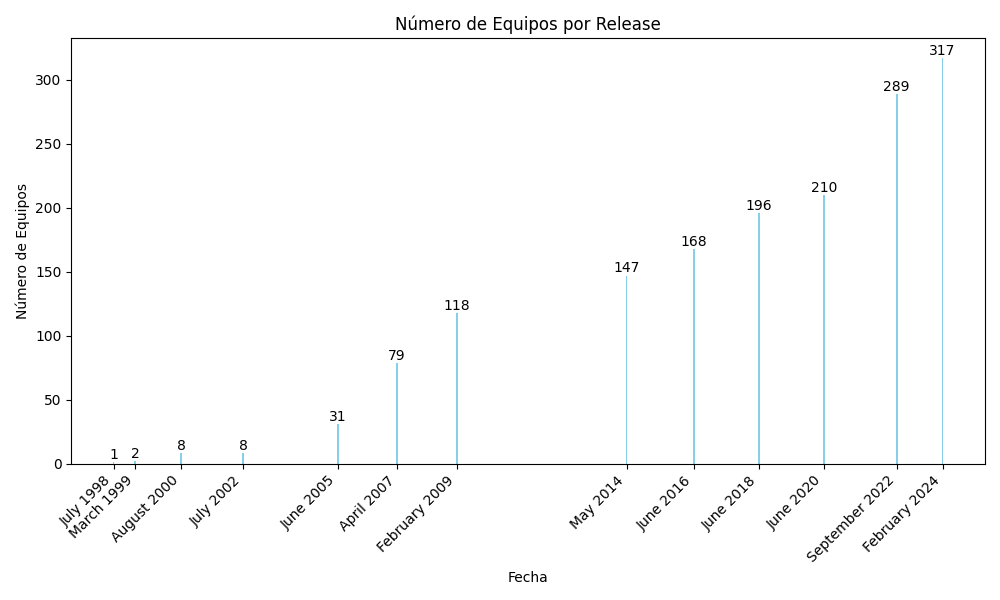
\includegraphics[width=15cm, keepaspectratio]{img/Figura3_buena_equipos.png}
	\caption{Equipos formados en cada release}
	\label{fig:equipos}
\end{figure}

Podemos apreciar observando la \textbf{Figura~\ref{fig:equipos}} la tendencia que sigue la creación de equipos. Es claramente ascendente llegando hasta los 317 en su último release de 2024.

Se distinguen cuatro fases.
\begin{itemize}
	\item  \textbf{Fase 1:} los 4 primeros releases conformados por muy pocos equipos con un máximo de ocho de 1998 a 2002. 
	
	\item  \textbf{Fase 2:} los 3 siguientes a la `Fase 1' cuentan con una subida sustancial de equipos llegando a un máximo de 118 de 2005 a 2009.
	
	\item  \textbf{Fase 3:} los 4 siguientes a la `Fase 2' cuentan con una subida en la conformación de equipos llegando a un máximo de 210 de 2014 a 2020.
	
	\item  \textbf{Fase 4:} los 2 siguientes a la `Fase 3' cuentan con una subida  llegando a un máximo de 317 de 2005 a 2009.
	
\end{itemize}

\section{¿Cuántos mantenedores de versiones anteriores permanecen activos?}
\label{sec:pregunta_3}

Como comentamos en las sección~\ref{sec:pregunta_1}, con el paso del tiempo hay mantenedores nuevos que entran al proyecto y también existen mantenedores que lo abandonan. Por ello nos preguntamos cuantos de los mantenedores anteriores siguen en los releases posteriores y cual es el porcentaje de los mismos comparando los releases.



Como queremos comparar (en valor absoluto) cuantos maintainers se mantienen de un release a los demás, realizamos otra query para ello.
Este es su resultado:
	

	
		
\begin{table}[htbp]
	\label{tab:tabla1}
	\centering
	\scalebox{0.6}{
		\begin{tabular}{|l|l|l|l|l|l|l|l|l|l|l|l|l|l|}
			\hline
			Release      & 1.Hamm & 2. Slink & 3.Potato & 4. Woody & 5. Sarge & 6. Etch & 7. Lenny & 8. Squeeze & 9. Wheezy & 10. Jessie & 11. Stretch & 12. Buster & 13. Bullseye \\ \hline
			1. Hamm      & 255                      & 242                      & 210                      & 155                      & 121                      & 98                       & 83                       & 71                       & 69                       & 64                       & 54                       & 48                       & 46            \\ \hline
			2. Slink     & \cellcolor[HTML]{000000} & 362                      & 314                      & 241                      & 186                      & 153                      & 132                      & 106                      & 95                       & 88                       & 73                       & 67                       & 64            \\ \hline
			3. Potato    & \cellcolor[HTML]{000000} & \cellcolor[HTML]{000000} & 530                      & 412                      & 300                      & 243                      & 198                      & 169                      & 151                      & 140                      & 125                      & 109                      & 101           \\ \hline
			4. Woody     & \cellcolor[HTML]{000000} & \cellcolor[HTML]{000000} & \cellcolor[HTML]{000000} & 986                      & 726                      & 576                      & 487                      & 410                      & 359                      & 333                      & 292                      & 268                      & 236           \\ \hline
			5. Sarge     & \cellcolor[HTML]{000000} & \cellcolor[HTML]{000000} & \cellcolor[HTML]{000000} & \cellcolor[HTML]{000000} & 1490                     & 1235                     & 1039                     & 855                      & 728                      & 668                      & 573                      & 519                      & 457           \\ \hline
			6. Etch      & \cellcolor[HTML]{000000} & \cellcolor[HTML]{000000} & \cellcolor[HTML]{000000} & \cellcolor[HTML]{000000} & \cellcolor[HTML]{000000} & 1760                     & 1483                     & 1231                     & 1055                     & 949                      & 805                      & 713                      & 628           \\ \hline
			7. Lenny     & \cellcolor[HTML]{000000} & \cellcolor[HTML]{000000} & \cellcolor[HTML]{000000} & \cellcolor[HTML]{000000} & \cellcolor[HTML]{000000} & \cellcolor[HTML]{000000} & 1971                     & 1647                     & 1418                     & 1266                     & 1076                     & 941                      & 829           \\ \hline
			8. Squeeze   & \cellcolor[HTML]{000000} & \cellcolor[HTML]{000000} & \cellcolor[HTML]{000000} & \cellcolor[HTML]{000000} & \cellcolor[HTML]{000000} & \cellcolor[HTML]{000000} & \cellcolor[HTML]{000000} & 2173                     & 1859                     & 1687                     & 1409                     & 1211                     & 1046          \\ \hline
			9. Wheezy    & \cellcolor[HTML]{000000} & \cellcolor[HTML]{000000} & \cellcolor[HTML]{000000} & \cellcolor[HTML]{000000} & \cellcolor[HTML]{000000} & \cellcolor[HTML]{000000} & \cellcolor[HTML]{000000} & \cellcolor[HTML]{000000} & 2286                     & 2029                     & 1712                     & 1470                     & 1253          \\ \hline
			10. Jessie   & \cellcolor[HTML]{000000} & \cellcolor[HTML]{000000} & \cellcolor[HTML]{000000} & \cellcolor[HTML]{000000} & \cellcolor[HTML]{000000} & \cellcolor[HTML]{000000} & \cellcolor[HTML]{000000} & \cellcolor[HTML]{000000} & \cellcolor[HTML]{000000} & 2468                     & 2082                     & 1778                     & 1511          \\ \hline
			11. Stretch  & \cellcolor[HTML]{000000} & \cellcolor[HTML]{000000} & \cellcolor[HTML]{000000} & \cellcolor[HTML]{000000} & \cellcolor[HTML]{000000} & \cellcolor[HTML]{000000} & \cellcolor[HTML]{000000} & \cellcolor[HTML]{000000} & \cellcolor[HTML]{000000} & \cellcolor[HTML]{000000} & 2412                     & 2051                     & 1742          \\ \hline
			12. Buster   & \cellcolor[HTML]{000000} & \cellcolor[HTML]{000000} & \cellcolor[HTML]{000000} & \cellcolor[HTML]{000000} & \cellcolor[HTML]{000000} & \cellcolor[HTML]{000000} & \cellcolor[HTML]{000000} & \cellcolor[HTML]{000000} & \cellcolor[HTML]{000000} & \cellcolor[HTML]{000000} & \cellcolor[HTML]{000000} & 2413                     & 2059          \\ \hline
			13. Bullseye & \cellcolor[HTML]{000000} & \cellcolor[HTML]{000000} & \cellcolor[HTML]{000000} & \cellcolor[HTML]{000000} & \cellcolor[HTML]{000000} & \cellcolor[HTML]{000000} & \cellcolor[HTML]{000000} & \cellcolor[HTML]{000000} & \cellcolor[HTML]{000000} & \cellcolor[HTML]{000000} & \cellcolor[HTML]{000000} & \cellcolor[HTML]{000000} & 2293          \\ \hline
		\end{tabular}
	}
	\caption{Valores absolutos de maintainers que permanecen activos en versiones posteriores}
\end{table}

	


	
	
	
	



	
	En la tabla~\ref{tab:tabla1} podemos ver cual es el valor absoluto de los maintainers de un release que se mantienen en el resto. Se lee de izquierda a derecha comparando el primero con el segundo, el primero con el tercero, el primero con el cuarto, etc.
	
	Analizando esta tabla podemos observar que, según avanzan los releases, disminuye el número de maintainers que aguantan en versiones posteriores.
	
	Ejecutamos una segunda query para observar los porcentajes de equipos de mantenedores:
	



\begin{table}[htbp]
	\label{tab:tabla2}
	\scalebox{0.6}{
		\begin{tabular}{|l|l|l|l|l|l|l|l|l|l|l|l|l|l|}
			\hline
			Release      & 1.Hamm & 2. Slink & 3.Potato & 4. Woody & 5. Sarge & 6. Etch & 7. Lenny & 8. Squeeze & 9. Wheezy & 10. Jessie & 11. Stretch & 12. Buster & 13. Bullseye \\ \hline
			1. Hamm      & 1 & 1 & 1 & 1 & 1 & 1 & 1 & 1 & 1 & 1 & 1 & 1 & 1 \\ \hline
			2. Slink     & \cellcolor[HTML]{000000} & 2 & 2 & 2 & 2 & 2 & 2 & 2 & 2 & 2 & 2 & 2 & 2 \\ \hline
			3. Potato    & \cellcolor[HTML]{000000} & \cellcolor[HTML]{000000} & 8 & 4 & 4 & 4 & 4 & 4 & 4 & 4 & 4 & 4 & 4 \\ \hline
			4. Woody     & \cellcolor[HTML]{000000} & \cellcolor[HTML]{000000} & \cellcolor[HTML]{000000} & 8 & 7 & 4 & 4 & 4 & 4 & 4 & 4 & 4 & 4 \\ \hline
			5. Sarge     & \cellcolor[HTML]{000000} & \cellcolor[HTML]{000000} & \cellcolor[HTML]{000000} & \cellcolor[HTML]{000000} & 31 & 26 & 25 & 22 & 21 & 21 & 19 & 18 & 18 \\ \hline
			6. Etch      & \cellcolor[HTML]{000000} & \cellcolor[HTML]{000000} & \cellcolor[HTML]{000000} & \cellcolor[HTML]{000000} & \cellcolor[HTML]{000000} & 79 & 68 & 62 & 53 & 49 & 47 & 41 & 40 \\ \hline
			7. Lenny     & \cellcolor[HTML]{000000} & \cellcolor[HTML]{000000} & \cellcolor[HTML]{000000} & \cellcolor[HTML]{000000} & \cellcolor[HTML]{000000} & \cellcolor[HTML]{000000} & 118 & 104 & 93 & 90 & 78 & 66 & 63 \\ \hline
			8. Squeeze   & \cellcolor[HTML]{000000} & \cellcolor[HTML]{000000} & \cellcolor[HTML]{000000} & \cellcolor[HTML]{000000} & \cellcolor[HTML]{000000} & \cellcolor[HTML]{000000} & \cellcolor[HTML]{000000} & 147 & 130 & 124 & 109 & 83 & 78 \\ \hline
			9. Wheezy    & \cellcolor[HTML]{000000} & \cellcolor[HTML]{000000} & \cellcolor[HTML]{000000} & \cellcolor[HTML]{000000} & \cellcolor[HTML]{000000} & \cellcolor[HTML]{000000} & \cellcolor[HTML]{000000} & \cellcolor[HTML]{000000} & 168 & 153 & 131 & 99 & 91 \\ \hline
			10. Jessie   & \cellcolor[HTML]{000000} & \cellcolor[HTML]{000000} & \cellcolor[HTML]{000000} & \cellcolor[HTML]{000000} & \cellcolor[HTML]{000000} & \cellcolor[HTML]{000000} & \cellcolor[HTML]{000000} & \cellcolor[HTML]{000000} & \cellcolor[HTML]{000000} & 196 & 168 & 130 & 119 \\ \hline
			11. Stretch  & \cellcolor[HTML]{000000} & \cellcolor[HTML]{000000} & \cellcolor[HTML]{000000} & \cellcolor[HTML]{000000} & \cellcolor[HTML]{000000} & \cellcolor[HTML]{000000} & \cellcolor[HTML]{000000} & \cellcolor[HTML]{000000} & \cellcolor[HTML]{000000} & \cellcolor[HTML]{000000} & 210 & 166 & 150 \\ \hline
			12. Buster   & \cellcolor[HTML]{000000} & \cellcolor[HTML]{000000} & \cellcolor[HTML]{000000} & \cellcolor[HTML]{000000} & \cellcolor[HTML]{000000} & \cellcolor[HTML]{000000} & \cellcolor[HTML]{000000} & \cellcolor[HTML]{000000} & \cellcolor[HTML]{000000} & \cellcolor[HTML]{000000} & \cellcolor[HTML]{000000} & 289 & 263 \\ \hline
			13. Bullseye & \cellcolor[HTML]{000000} & \cellcolor[HTML]{000000} & \cellcolor[HTML]{000000} & \cellcolor[HTML]{000000} & \cellcolor[HTML]{000000} & \cellcolor[HTML]{000000} & \cellcolor[HTML]{000000} & \cellcolor[HTML]{000000} & \cellcolor[HTML]{000000} & \cellcolor[HTML]{000000} & \cellcolor[HTML]{000000} & \cellcolor[HTML]{000000} & 317 \\ \hline
	\end{tabular}}
	\caption{Valores absolutos de equipos que permanecen activos en versiones}
\end{table}





En la tabla~\ref{tab:tabla2} se observa la evolución de los equipos o grupos que se mantienen de una versión en las posteriores en porcentajes.

Podemos ver como los grupos creados en los releases Hamm y Slink se mantienen en todos los releases pero en los demás va disminuyendo según se lanzan nuevas versiones.

Esto puede deberse a la creación de nuevos equipos que sustituyan a los anteriores para la mejora de eficiencia al mantener paquetes.

También quisimos responder a la pregunta de cuál es la vida media de un maintainer, es decir, cuando se reduce a la mitad el número de maintainer de un release. 

Ejecutamos un query en la que obtenemos dicho valor el cual tiene como resultado 3.5 releases.

Sabemos que no todos los maintainers de una versión se mantienen en las siguientes. Pero, ¿hay maintainers que comenzaron en la primera versión y hoy en día siguen activos?

Para resolverlo ejecutamos una query que, coge todos los maintainers únicos de cada versión y realiza un \textbf{set~\cite{ellibrodepython:_set}}.

Un `set' es como una lista o un array pero con la peculiaridad de que sus items deben ser únicos, justo lo que necesitamos para resolver esta pregunta.

Una vez tengamos un `set' con los maintainers de la primera versión, realizamos la \textbf{intersección}~\cite{medium:_intersection} con el `set' de la segunda versión, y así sucesivamente. 

Con una intersección entre las versiones conseguimos quedarnos únicamente con los maintainers que se repiten en todas las versiones. Estos son los que permanecerán activos.

Ejecutando la query obtenemos estos resultados:
\begin{multicols}{3}
	\begin{itemize}
		\item Manoj Srivastava
		\item Roderick Schertler
		\item Davide G. M. Salvetti
		\item Anthony Fok
		\item Roberto Lumbreras
		\item Juan Cespedes
		\item Riku Voipio
		\item Michael Meskes
		\item Craig Small
		\item Anselm Lingnau
		\item Miquel van Smoorenburg
		\item John Goerzen
		\item Dirk Eddelbuettel
		\item Martin Buck
		\item Paul Slootman
		\item Marco d'Itri
		\item Jaldhar H. Vyas
		\item Bdale Garbee
		\item Matthias Klose
		\item Martin Schulze
		\item Joel Rosdahl
		\item Fredrik Hallenberg
		\item Yann Dirson
		\item Hakan Ardo
		\item Philip Hands
		\item Craig Sanders
		\item Norbert Veber
	\end{itemize}
\end{multicols}


En esta lista/set encontramos los maintainers que llevan desde el inicio manteniendo paquetes de diferentes versiones en Debian.

\section{¿Cuál es el aporte de los mantenedores que permanecen en versiones posteriores?}
\label{sec:pregunta_4}
Tras haber obtenido los maintainers que han estado activos en todas las versiones, queremos conocer que paquetes mantienen de cada versión.

Diseñamos una query para buscar en las BBDD que paquetes tienen, en el campo maintainer, el nombre de alguno de los mantenedores de la lista anterior. Con un bucle vamos recorriendo cada BBDD y almacenamos en arrays los resultados de los paquetes de cada maintainer.

\begin{verbatim}
	"SELECT DISTINCT p.nombre FROM package p INNER JOIN maintainer m ON "
	"p.maintainer_id = m.id WHERE m.nombre = %s"
\end{verbatim}
Una vez ejecutada dicha query, se muestran unos ejemplos de los resultados en la tabla.

Podemos observar que, en los tres ejemplos expuestos en la tabla, hay paquetes que se repiten varias veces en un mismo mantenedor. Esto se debe a que, como son maintainers que llevan desde el inicio de Debian, tienen asociados una serie de paquetes que mantendrán a lo largo de las próximas versiones a menos que abandonen o deje de interesar su mantenimiento.

	
	\begin{table}[h!]
		\centering
		\begin{tabular}{|l|p{10cm}|}
			\hline
			\textbf{Maintainer} & \textbf{Paquetes} \\
			\hline
			Norbert Veber \textless{}nveber@debian.org\textgreater{} & bplay, xinetd, bplay, radiusd-cistron, xinetd, radiusd-cistron, gabber, gcdb, gnome-media, gphone, radiusd-cistron, screem, gkrellweather, imms, radiusd-cistron, gkrellweather, imms, rig, gkrellweather, rig, gkrellweather, rig, gkrellweather, rig, gkrellweather, rig, gkrellweather, rig, gkrellweather, rig, gkrellweather, rig \\
			\hline
			Anselm Lingnau \textless{}lingnau@debian.org\textgreater{} & abc2ps, abcmidi, abc2ps, abcmidi, xtartan, abc2ps, abcmidi, bwidget, tkdvi, xtartan, abc2ps, abcmidi, bwidget, tkdvi, xtartan, abc2ps, abcm2ps, abcmidi, bwidget, tkdvi, xtartan, abcm2ps, abcmidi, bwidget, tkdvi, xtartan, abcm2ps, abcmidi, tkdvi, xtartan, abcm2ps, abcmidi, abcm2ps, abcmidi, abcm2ps, abcm2ps, abcm2ps, abcm2ps \\
			\hline
			Davide G. M. Salvetti \textless{}salve@debian.org\textgreater{} & auctex, lacheck, witalian, auctex, lacheck, witalian, auctex, lacheck, statnews, witalian, auctex, lacheck, mimefilter, statnews, witalian, auctex, lacheck, mailcrypt, mimefilter, statnews, witalian, auctex, lacheck, mailcrypt, mimefilter, statnews, witalian, auctex, lacheck, mailcrypt, mimefilter, statnews, witalian, auctex, lacheck, mailcrypt, mimefilter, statnews, witalian, auctex, lacheck, mailcrypt, mimefilter, statnews, witalian, auctex, lacheck, mailcrypt, mimefilter, statnews, witalian, auctex, lacheck, mimefilter, statnews, witalian, auctex, lacheck, mimefilter, statnews, witalian, auctex, lacheck, mimefilter, statnews, witalian \\
			\hline
		\end{tabular}
		\caption{Lista de paquetes por maintainer}
	\end{table}







Se observa que cada mantenedor tiene muchos paquetes debido a su larga vida dentro del proyecto por lo que no podemos sacar todos los resultados ya que son muy extensos.


\section{¿Qué sucede con los paquetes mantenidos por los mantenedores que abandonan el proyecto?}
\label{sec:pregunta_5}
Hemos visto en la sección~\ref{sec:pregunta_4} cuantos mantenedores permanecen activos y cuales han sido sus aportaciones a lo largo de la evolución de Debian. 
Pero, ¿qué ocurre con los paquetes asociados a un maintainer que abandona el proyecto?
Debe existir un método de control u organización para estos casos en los que no se puede dejar un paquete sin maintainer.
Para ello, cogemos a uno de los maintainers que no aparezcan en la sección anterior y realizamos un seguimiento del paquete para ver que ocurre con él.

Cogemos como ejemplo a el maintainer \textbf{Martin Albisetti} y ejecutamos una query que devuelve los paquetes mantenidos por \textbf{Martin Albisetti} junto con la versión en la que se encuentra.

% Please add the following required packages to your document preamble:
% \usepackage[table,xcdraw]{xcolor}
% Beamer presentation requires \usepackage{colortbl} instead of \usepackage[table,xcdraw]{xcolor}
% Please add the following required packages to your document preamble:
% \usepackage[table,xcdraw]{xcolor}
% Beamer presentation requires \usepackage{colortbl} instead of \usepackage[table,xcdraw]{xcolor}
% Please add the following required packages to your document preamble:
% \usepackage[table,xcdraw]{xcolor}
% Beamer presentation requires \usepackage{colortbl} instead of \usepackage[table,xcdraw]{xcolor}
% Please add the following required packages to your document preamble:
% \usepackage[table,xcdraw]{xcolor}
% Beamer presentation requires \usepackage{colortbl} instead of \usepackage[table,xcdraw]{xcolor}
\begin{table}[h]
	\begin{tabular}{|c|cc|}
		\hline
		\rowcolor[HTML]{FFFE65} 
		Releases        & \multicolumn{2}{c|}{\cellcolor[HTML]{FFFE65}Packages} \\ \hline
		7.lenny\_main   & \multicolumn{1}{c|}{2vcard}        & exifprobe        \\ \hline
		8.squeeze\_main & \multicolumn{1}{c|}{2vcard}        & exifprobe        \\ \hline
		9.wheezy\_main  & \multicolumn{1}{c|}{2vcard}        & exifprobe        \\ \hline
		10.jessie\_main & \multicolumn{2}{c|}{2vcard}                           \\ \hline
	\end{tabular}
\end{table}

Como podemos ver en la tabla, este maintainer tiene asociados dos paquetes en los releases \textbf{Lenny, Squeeze y Wheezy}, en el release \textbf{Jessie} solo mantiene uno y abandona el proyecto para releases posteriores.

Ahora vamos a realizar un seguimiento a dichos paquetes en todos los releases obteniendo quien es la persona o equipo que los mantiene ejecutando otra query.
 
 % Please add the following required packages to your document preamble:
 % \usepackage[table,xcdraw]{xcolor}
 % Beamer presentation requires \usepackage{colortbl} instead of \usepackage[table,xcdraw]{xcolor}
 \begin{table}[]
 	\begin{tabular}{|l|l|l|}
 		\hline
 		\rowcolor[HTML]{FFFE65} 
 		Release           & Package   & Maintainer            \\ \hline
 		\rowcolor[HTML]{FFFFFF} 
 		7.lenny\_main     & 2vcard    & Martin Albisetti      \\ \hline
 		\rowcolor[HTML]{FFFFFF} 
 		7.lenny\_main     & exifprobe & Martin Albisetti      \\ \hline
 		\rowcolor[HTML]{FFFFFF} 
 		8.squeeze\_main   & 2vcard    & Martin Albisetti      \\ \hline
 		\rowcolor[HTML]{FFFFFF} 
 		8.squeeze\_main   & exifprobe & Martin Albisetti      \\ \hline
 		\rowcolor[HTML]{FFFFFF} 
 		9.wheezy\_main    & 2vcard    & Martin Albisetti      \\ \hline
 		\rowcolor[HTML]{FFFFFF} 
 		9.wheezy\_main    & exifprobe & Martin Albisetti      \\ \hline
 		\rowcolor[HTML]{FFFFFF} 
 		10.jessie\_main   & 2vcard    & Martin Albisetti      \\ \hline
 		\rowcolor[HTML]{FFFFFF} 
 		10.jessie\_main   & exifprobe & Debian Forensics      \\ \hline
 		\rowcolor[HTML]{FFFFFF} 
 		11.stretch\_main  & 2vcard    & Riley Baird           \\ \hline
 		\rowcolor[HTML]{FFFFFF} 
 		11.stretch\_main  & exifprobe & Debian Forensics      \\ \hline
 		\rowcolor[HTML]{FFFFFF} 
 		12.buster\_main   & 2vcard    & Riley Baird           \\ \hline
 		\rowcolor[HTML]{FFFFFF} 
 		12.buster\_main   & exifprobe & Debian Security Tools \\ \hline
 		\rowcolor[HTML]{FFFFFF} 
 		13.bullseye\_main & 2vcard    & Debian QA Group       \\ \hline
 		\rowcolor[HTML]{FFFFFF} 
 		13.bullseye\_main & exifprobe & Debian Security Tools \\ \hline
 	\end{tabular}
 \end{table}
 
En esta tabla se puede observar que, a partir de la versión \textbf{Jessie}, el paquete \textbf{exifprobe} comienza a mantenerse por un grupo de Debian.
En el release \textbf{Stretch y Buster} el paquete \textbf{2vcard} es mantenido por \textbf{Riley Baird} mientras que \textbf{exifprobe} sigue mantenido por el grupo anterior.
En \textbf{Buster} cambia el paquete \textbf{exifprobe} de mantenedor a otro grupo de seguridad de Debian.
Y finalmente se asignan los dos paquetes a grupos Debian.

Podemos ver los paquetes \textbf{huérfanos} se asocian a otros maintainers o a grupos para que trabajen en ellos. 

También hay paquetes que dejan de usarse de una versión a otra aunque el maintainer no haya abandonado el proyecto.

Observando otros ejemplos vemos una clara tendencia a la mantención de dichos paquetes por grupos Debian a partir de la versión Buster.

Como podemos ver en la \textbf{Figura~\ref{fig:equipos}}, a partir de la versión Buster hay un claro aumento en el número de equipos Debian, de 210 a 289, por lo que es lógico pensar que se han distribuido estos paquetes entre los diferentes grupos.

También se refleja en la \textbf{Figura~\ref{fig:mantenedores}} que en cada versión hay un aumento de los mantenedores hasta la versión Buster en la que observamos una tendencia de bajada en el número de los mismos.

Por ello podemos pensar que, hasta la versión Buster, se asignaban a maintainers pero a partir de dicha release comenzaron a organizarse en equipos y repartieron dichos paquetes entre los mismos.


\section{¿Los paquetes más importantes y de uso común son mantenidos por mantenedores más experimentados?}
\label{sec:pregunta_6}

Para resolver esta pregunta debemos conocer cuales son los paquetes más importantes y usados de Debian. Entramos en la página de Debian Popcon~\cite{debian:_popcon}, accedemos a las estadísticas de \textbf{la suma de paquetes ordenados}.Tras esto nos fijamos en el campo \textbf{vote} que indica el \textbf{número de personas que usan este paquete regularmente}. Estos paquetes son los que consideramos \textbf{importantes} como se muestra en la tabla.


	\begin{table}[h!]
		\centering
		\begin{tabular}{|c|l|r|r|r|r|r|}
			\hline
			\#rank & name & inst & vote & old & recent & no-files \\
			\hline
			1 & Not in sid & 19992113 & 2857277 & 4663481 & 395618 & 12075737 \\
			\hline
			2 & util-linux & 2890959 & 1641090 & 692861 & 339533 & 217115 \\
			\hline
			3 & systemd & 1998462 & 1587252 & 149416 & 169750 & 92044 \\
			\hline
			4 & gnupg2 & 2248600 & 1580116 & 356679 & 178782 & 133023 \\
			\hline
			5 & libxcb & 2578180 & 1237197 & 334256 & 201889 & 804838 \\
			\hline
			6 & dbus & 1199936 & 953625 & 123986 & 120765 & 1560 \\
			\hline
			7 & krb5 & 1237409 & 858656 & 68086 & 69262 & 241405 \\
			\hline
			8 & gcc-14 & 1911702 & 788522 & 537396 & 164995 & 420789 \\
			\hline
			9 & libblockdev & 904164 & 705667 & 263 & 104876 & 93358 \\
			\hline
			10 & libreoffice & 2935606 & 670532 & 1480947 & 507072 & 277055 \\
			\hline
			11 & pam & 955649 & 668089 & 207763 & 79222 & 575 \\
			\hline
		\end{tabular}
		\caption{Paquetes Popcon más usados ordenados por vote.}
	\end{table}



El paquete \textbf{Not in sid} no aparece en ninguna versión o release de Debian.
Debian tiene varias ramas de desarrollo:
\begin{itemize}
	\item \textbf{Unstable o Sid}: se desarrollan activamente los paquetes de Debian. Pueden tener errores y no se garantiza su estabilidad. Es usada principalmente por desarrolladores y usuarios avanzados para probar las últimas versiones.
	\item \textbf{Testing}: se prueban los paquetes que probablemente formarán parte de la próxima versión estable de Debian.
	\item \textbf{Stable}: contiene paquetes que han sido probados extensivamente y se consideran estables para el uso diario.
	
\end{itemize}

Este paquete \textbf{Not in sid} no está disponible en la rama unstable de Debian. Esto indica que el paquete no está en la fase de desarrollo activo o que no cumple con los estándares para ser incluido en la rama unstable.

Tras encontrar los nombres de los paquetes más importantes, diseñamos una query para obtener que maintainers son los que mantienen estos paquetes. Y al ejecutarla estos son los resultados:


	\begin{longtable}{|c|c|c|}
		\caption{Información de paquetes encontrados} \label{tab:packages_info} \\
		\hline
		\textbf{Paquete} & \textbf{Base de datos} & \textbf{Maintainer} \\
		\hline
		\endfirsthead
		
		\multicolumn{3}{c}%
		{{\tablename\ \thetable{} -- continuación de la página anterior}} \\
		\hline
		\textbf{Paquete} & \textbf{Base de datos} & \textbf{Maintainer} \\
		\hline
		\endhead
		
		\hline
		\endfoot
		
		\hline
		\endlastfoot
		
		util-linux
		& 1.hamm\_main & Guy Maor \\
		& 2.slink\_main & Vincent Renardias \\
		& 3.potato\_main & Vincent Renardias \\
		& 4.woody\_main & LaMont Jones \\
		& 5.sarge\_main & LaMont Jones \\
		& 6.etch\_main & LaMont Jones \\
		& 7.lenny\_main & LaMont Jones \\
		& 8.squeeze\_main & LaMont Jones \\
		& 9.wheezy\_main & LaMont Jones \\
		& 10.jessie\_main & Debian util-linux Maintainers \\
		& 11.stretch\_main & Debian util-linux Maintainers \\
		& 12.buster\_main & LaMont Jones \\
		& 13.bullseye\_main & util-linux packagers \\
		\hline
		gnupg2 & 5.sarge\_main & Matthias Urlichs \\
		& 6.etch\_main & Eric Dorland \\
		& 7.lenny\_main & Eric Dorland \\
		& 8.squeeze\_main & Eric Dorland \\
		& 9.wheezy\_main & Eric Dorland \\
		& 10.jessie\_main & Debian GnuPG Maintainers \\
		& 11.stretch\_main & Debian GnuPG Maintainers \\
		& 12.buster\_main & Debian GnuPG Maintainers \\
		& 13.bullseye\_main & Debian GnuPG Maintainers \\
		\hline
		systemd & 9.wheezy\_main & Tollef Fog Heen \\
		& 10.jessie\_main & Debian systemd Maintainers \\
		& 11.stretch\_main & Debian systemd Maintainers \\
		& 12.buster\_main & Debian systemd Maintainers \\
		& 13.bullseye\_main & Debian systemd Maintainers \\
		\hline
		libxcb & 7.lenny\_main & XCB Developers \\
		& 8.squeeze\_main & XCB Developers \\
		& 9.wheezy\_main & XCB Developers \\
		& 10.jessie\_main & XCB Developers \\
		& 11.stretch\_main & Debian X Strike Force \\
		& 12.buster\_main & Debian X Strike Force \\
		& 13.bullseye\_main & Debian X Strike Force \\
		\hline
		dbus & 5.sarge\_main & D-Bus Maintainance Team \\
		& 6.etch\_main & Utopia Maintenance Team \\
		& 7.lenny\_main & Utopia Maintenance Team \\
		& 8.squeeze\_main & Utopia Maintenance Team \\
		& 9.wheezy\_main & Utopia Maintenance Team \\
		& 10.jessie\_main & Utopia Maintenance Team \\
		& 11.stretch\_main & Utopia Maintenance Team \\
		& 12.buster\_main & Utopia Maintenance Team \\
		& 13.bullseye\_main & Utopia Maintenance Team \\
		\hline
		krb5 & 4.woody\_main & Sam Hartman \\
		& 5.sarge\_main & Sam Hartman \\
		& 6.etch\_main & Sam Hartman \\
		& 7.lenny\_main & Sam Hartman \\
		& 8.squeeze\_main & Sam Hartman \\
		& 9.wheezy\_main & Sam Hartman \\
		& 10.jessie\_main & Sam Hartman \\
		& 11.stretch\_main & Sam Hartman \\
		& 12.buster\_main & Sam Hartman \\
		& 13.bullseye\_main & Sam Hartman \\
		\hline
		libblockdev & 12.buster\_main & Utopia Maintenance Team \\
		& 13.bullseye\_main & Utopia Maintenance Team \\
		\hline
		libreoffice & 9.wheezy\_main & Debian LibreOffice Maintainers \\
		& 10.jessie\_main & Debian LibreOffice Maintainers \\
		& 11.stretch\_main & Debian LibreOffice Maintainers \\
		& 12.buster\_main & Debian LibreOffice Maintainers \\
		& 13.bullseye\_main & Debian LibreOffice Maintainers \\
		\hline
		avahi & 6.etch\_main & Utopia Maintenance Team \\
		& 7.lenny\_main & Utopia Maintenance Team \\
		& 8.squeeze\_main & Utopia Maintenance Team \\
		& 9.wheezy\_main & Utopia Maintenance Team \\
		& 10.jessie\_main & Utopia Maintenance Team \\
		& 11.stretch\_main & Utopia Maintenance Team \\
		& 12.buster\_main & Utopia Maintenance Team \\
		& 13.bullseye\_main & Utopia Maintenance Team \\
		\hline
	\end{longtable}


Tras estos resultados, en los que se muestran los releases donde se encuentran estos paquetes y los maintainers asociados a los mismos, creamos una query que coja todos estos maintainers (de forma única) y compruebe si son expertos o no basándonos en la \textbf{vida media}.

La \textbf{vida media} de un maintainer es la suma de el número de releases en los que se encuentran cada maintainer dividido entre el número total de maintainers únicos. 

Esto lo calculamos con otra query y nos devuelve como resultado que el número de apariciones de los maintainers es \textbf{21.409}, el número total de maintainers es \textbf{6.052} y la media de apariciones de un maintainer es \textbf{3.54}.

A partir de esta vida media podemos conocer si los maintainers que están asociados a los paquetes más importantes son \textbf{expertos} o no.

Comparamos las apariciones de cada uno de los maintainers anteriores con la vida media y diseñamos una query que devuelva si es experto. Estos son los resultados:

	\begin{itemize}
		\item El maintainer \textbf{Guy Maor} es un experto con presencia en 4 bases de datos (superando la media total).
		\item El maintainer \textbf{Vincent Renardias} es un experto con presencia en 4 bases de datos (superando la media total).
		\item El maintainer \textbf{LaMont Jones} es un experto con presencia en 11 bases de datos (superando la media total).
		\item El maintainer \textbf{Tollef Fog Heen} es un experto con presencia en 11 bases de datos (superando la media total).
		\item El maintainer \textbf{Eric Dorland} es un experto con presencia en 10 bases de datos (superando la media total).
		\item El maintainer \textbf{Sam Hartman} es un experto con presencia en 10 bases de datos (superando la media total).
		\item El maintainer \textbf{Matthias Urlichs} es un experto con presencia en 9 bases de datos (superando la media total).
		\item El maintainer \textbf{Debian X Strike Force} es un experto con presencia en 9 bases de datos (superando la media total).
		\item El maintainer \textbf{Utopia Maintenance Team} es un experto con presencia en 8 bases de datos (superando la media total).
		\item El maintainer \textbf{XCB Developers} es un experto con presencia en 5 bases de datos (superando la media total).
		\item El maintainer \textbf{Debian LibreOffice Maintainers} es un experto con presencia en 5 bases de datos (superando la media total).
		\item El maintainer \textbf{Debian systemd Maintainers} es un experto con presencia en 4 bases de datos (superando la media total).
		\item El maintainer \textbf{Debian GnuPG Maintainers} es un experto con presencia en 4 bases de datos (superando la media total).
		\item El maintainer \textbf{D-Bus Maintainance Team} NO es un experto con presencia en 1 base de datos.
		\item El maintainer \textbf{util-linux packagers} NO es un experto con presencia en 1 base de datos.
	\end{itemize}

Como se observa en los resultados, hay 13 maintainers expertos y 2 no expertos en un total de 15 maintainers. Los que definimos como no expertos son grupos recientes formados por Debian y esta puede ser la explicación de porque no llevan tantas versiones activos.
%%%%%%%%%%%%%%%%%%%%%%%%%%%%%%%%%%%%%%%%%%%%%%%%%%%%%%%%%%%%%%%%%%%%%%%%%%%%%%%%
%%%%%%%%%%%%%%%%%%%%%%%%%%%%%%%%%%%%%%%%%%%%%%%%%%%%%%%%%%%%%%%%%%%%%%%%%%%%%%%%
% CONCLUSIONES %
%%%%%%%%%%%%%%%%%%%%%%%%%%%%%%%%%%%%%%%%%%%%%%%%%%%%%%%%%%%%%%%%%%%%%%%%%%%%%%%%

\cleardoublepage
\chapter{Conclusiones}
\label{chap:conclusiones}
En esta sección comentaremos cuales fueron los resultados del estudio realizado hace veinte años visto en la subsección~\ref{subsec:articulo debian} comparados con los obtenidos en este proyecto. De esta forma, podremos aportar las conclusiones adecuadas.

\section{Conclusiones a las cuestiones planteadas}
\label{sec:conclusiones-cuestiones}
Como vimos en el capitulo de resultados~\ref{chap:resultados} obtuvimos una serie de respuestas a las preguntas planteadas y, en consecuencia, aportaremos las conclusiones necesarias.

\subsection{Conclusiones: ¿Cuántos mantenedores tiene Debian y cómo cambia este número con el tiempo?}
\label{subsec:conclusion_1}
En el \textbf{estudio anterior~\cite{robles05:_debian}} llegaron a la conclusión de que había un aumento en el número de maintainers de casi un \textbf{35\%} en cada release. También un aumento, a mayor escala, en el número de paquetes de cada release. Por ello pensaron que podía deberse a una mayor eficiencia de los maintainers por el desarrollo de nuevas tecnologías o en las prácticas de desarrollo.

Los resultados obtenidos en este proyecto difieren en ciertos aspectos del estudio anterior.
\begin{itemize}
	\item Los porcentajes de aumento o disminución de maintainers entre los diferentes releases vistos en la \textbf{Figura~\ref{fig:mantenedores}} son: 
	\begin{enumerate}
		\item Subida del 41\%.
		\item Subida del 46\%.
		\item Subida del 86\%.
		\item Subida del 51\%.
		\item Subida del 18\%.
		\item Subida del 11\%.
		\item Subida del 10\%.
		\item Subida del 5\%.
		\item Subida del 7\%.
		\item Bajada del 2\%.
		\item Se mantiene con un ligero aumento de 2 maintainers.
		\item Bajada del 5\%.
	\end{enumerate}
\end{itemize}

La tendencia ha sido ascendente hasta la versión \textbf{10 Jessie} en la cual empezó a mantenerse e incluso a descender en número. Esto puede deberse a la creación de grupos los cuales se organizaban y distribuían el trabajo entre sí. Esta conclusión está respaldada por la \textbf{Figura~\ref{fig:paquetes}} en la que se muestra un gran número de paquetes según evoluciona Debian. Por ello, no tendría sentido la disminución de los maintainer con el aumento de los paquetes para que siga siendo una distribución estable. 

\subsection{Conclusiones: ¿Existe una tendencia hacia la formación de equipos de mantenedores?}
\label{subsec:conclusion_2}
En el \textbf{estudio anterior~\cite{robles05:_debian}} se refleja que ha habido un claro aumento en el número de paquetes que mantiene un maintainer y que esto se debe a que se ha obtenido una mayor conciencia sobre la imprevisibilidad de los voluntarios formando equipos organizados los cuales mantengan dichos paquetes.

Los resultados de este proyecto cuadran con el estudio. Como se observa en la \textbf{Figura~\ref{fig:equipos}} hay un aumento exponencial en la creación de equipos. En el release 10 Jessie se observa un elevado aumento de 210 a 289 que coincide con la disminución de los maintainers y con el aumento del número de paquetes. Con ello concluimos que hay una clara tendencia a la formación de grupos y esto resuelve la pregunta anterior~\ref{subsec:conclusion_1}.

\subsection{Conclusiones: ¿Cuántos mantenedores de versiones anteriores permanecen activos?}
\label{subsec:conclusion_3}
En el \textbf{estudio anterior~\cite{robles05:_debian}} se refleja que hay un claro descenso de los maintainers desde la primera versión que se mantienen en adelante. 
En el estudio de las primeras cuatro versiones se observa que ha bajado la aportación de los mismos y solo quedan (desde la primera versión) un 55\% de los mismos. Se intentó calcular la vida media de los maintainers, es decir, cuando su número baja hasta la mitad y se pronóstico que se daría al rededor de 7.5 años.

Las causas pueden ser por agotamiento pero estudios sobre recursos humanos dictan que se motivarían proyectos de software libre que ampliarían la vida media de los maintainers. 

En este proyecto obtuvimos dos tablas en las que se observa la disminución de aportaciones de los maintainers y grupos a lo largo de las diferentes versiones.

Por ello se calculó la vida media de cada uno que consta de 3.5 releases. Calculando en cuantos años se lanza un release obtenemos que de media es cada 2.16 años. Si vemos el tiempo en años en el que se cumple la vida media de un maintainer se obtiene que son 7.5 años por lo que la conclusión que se obtuvo en el estudio~\cite{robles05:_debian} coincide veinte años después.

\subsection{Conclusiones: ¿Cuál es el aporte de los mantenedores que permanecen en versiones posteriores?}
\label{subsec:conclusion_4}

En el \textbf{estudio anterior~\cite{robles05:_debian}} se refleja que, aunque el pensamiento inicial era que los mantenedores expertos tendrían más carga de trabajo, tienen números similares a maintainers más nuevos.

En este proyecto consideramos maintainers activos a los que llevan desde su primera versión hasta día de hoy en Debian. Como pudimos ver en los resultados, cada maintainer tiene asociado un gran conjunto de paquetes distribuidas entre todos los releases en los que se les asignaron.

Si nos fijamos en este dato podemos ver que estos maintainers mantienen muchos más paquetes que el resto pero hay que entender que esto es debido a que llevan desde el inicio.

Si los comparamos dentro de la misma versión, encontraremos resultados similares entre todos los maintainers por lo que la conclusión final coincide con la del estudio~\cite{robles05:_debian}. 

\subsection{Conclusiones: ¿Cuál es el aporte de los mantenedores que permanecen en versiones posteriores?}
\label{subsec:conclusion_5}

En el \textbf{estudio anterior~\cite{robles05:_debian}} se refleja que cuando los mantenedores abandonan un proyecto, sus paquetes quedan huérfanos. 

Más del 60\% de estos paquetes son adoptados en todas las versiones estudiadas, mostrando un proceso de regeneración natural en Debian. Sin embargo, el número de paquetes huérfanos crece más rápidamente que el de los adoptados, lo que sugiere que muchos paquetes no se mantienen en futuras versiones. 

Además, es importante establecer mecanismos para evitar la introducción de paquetes insostenibles a largo plazo. Los proyectos con más desarrolladores tienen mayores probabilidades de mantenerse activos.

En este proyecto realizamos el seguimiento a un paquete de un maintainer específico que abandonó el proyecto. Pudimos observar que, los dos paquetes que tenía asociados, fueron adoptados por otros maintainers o grupos por lo que se mantienen en la actualidad. También entendimos que, al formarse una gran cantidad de grupos Debian, se están empezando a adoptar por dichos grupos los cuales se distribuyen organizadamente y con sus estándares los diferentes paquetes.

\subsection{Conclusiones: ¿Los paquetes más importantes y de uso común son mantenidos por mantenedores más experimentados?}
\label{subsec:conclusion_6}

En el \textbf{estudio anterior~\cite{robles05:_debian}}, se usaron datos del Concurso de Popularidad de Debian para investigar si los paquetes más importantes son mantenidos por voluntarios más experimentados.

Al analizar el número de instalaciones y uso regular por mantenedor, concluyen que los voluntarios más experimentados mantienen los paquetes más frecuentemente instalados y utilizados. Esto es evidente en todas las versiones de Debian, excepto en la 2.2, que tiene valores más altos que la 2.1, indicando una actividad inusual de los mantenedores de esa época.

Esto también sugiere que muchos componentes esenciales de Debian se introdujeron en las primeras versiones, mientras que los nuevos paquetes son mayoritariamente complementos y software menos utilizados.

En este proyecto volvimos a coger los datos de los paquetes del Concurso de Popularidad de Debian. Diseñamos una query que devolviera que mantenedor o mantenedores tenían asignados los diez paquetes más usados y comparamos si eran expertos (comparando su vida con la vida media de 3.5 releases obtenida anteriormente).

Esto nos aportó un resultado de 13 expertos y 2 no expertos sobre un total de 15. Con esto podemos concluir que los paquetes más importantes de dicha distribución están asignados a los expertos.




\section{Consecución de objetivos}
\label{sec:consecucion-objetivos}

En este proyecto se ha cumplido el objetivo general basado en poder responder a las preguntas planteadas en el estudio de Debian. Esto ha sido posible gracias a los diferentes objetivos específicos planteados:

\begin{itemize}
	\item \textbf {Diseñar el diagrama entidad relación.} Este objetivo fue posible gracias al estudio de los diferentes paquetes y comprender las relaciones entre los atributos de los mismos. Este objetivo era el más importante ya que de él dependen los objetivos posteriores.
	Se encontraron ciertas dificultades para el diseño del diagrama debido a que esta formado por una entidad principal que acoge todas las demás. Hubo que adaptarlo para que en un folio se pudiera representar el mismo junto con sus tablas SQL.
	.
	\item \textbf {Crear la base de datos.} Este objetivo se separó en dos fases:
	\begin{enumerate}
		
		\item \textbf{Crear las BBDD de cada release.} Se realizó de forma manual en el programa MySQL Work Bench.
		
		\item \textbf{Crear las tablas SQL} Se realizó en PyCharm mediante un script. Fue algo tedioso debido a tener que analizar las diferentes relaciones entre entidades y añadir de forma correcta sus Primary Key y Foreing Key. También hubo tablas que no se podían relacionar entre sí y se tuvieron que diseñar tablas intermedias.
		
	\end{enumerate}
	\item \textbf {Inserción de los datos.} Se realizó en Pycharm mediante un script. Este fue el objetivo con mayor dificultad debido a problemas al insertar dichos datos y al volumen de los mismos. Una vez realizado de forma correcta fue esencial para tener los datos estructurados y organizados de tal forma que se puedan consultar fácil y rápidamente.
	
	\item \textbf {Formular las Queries.} Se realizó en Pycharm mediante un script. Tuvimos que mezclar lenguaje Python con SQL para poder diseñar bien las queries y que se ejecutaran para todas las BBDD mediante bucles. El diseño fue lo más problemático debido a que hay que entender correctamente lo que se quiere resolver para poder aplicar un algoritmo que funcione. 
	
	
	\item \textbf {Crear las tablas y gráficas.} Se realizó en Pycharm mediante un script. Una vez obtenidos los resultados con las queries, se usan los mismos para plasmarlos en gráficas o tablas. La mayor dificultad encontrada en este objetivo fue la inserción de un eje x temporal de forma que las gráficas quedaran espaciadas según el tiempo en el que se lanzó cada release.
\end{itemize}


\section{Aplicación de lo aprendido}
\label{sec:aplicacion}

Este proyecto no hubiera sido posible sin los conocimientos obtenidos en diferentes asignaturas del Grado en Ingeniería de Tecnologías de Telecomunicación.

Las más relacionadas con este proyecto son: 

\begin{itemize}
	\item \textbf {Ingeniería de Sistemas de Información.} Esta asignatura me aportó los conocimientos necesarios sobre diagramas entidad - relación y lenguaje SQL para poder realizar las queries y como relacionar las tablas de las bases de datos.
	
	\item \textbf {Sistemas Operativos.} Aunque el lenguaje usado fuera C y se basara en un lenguaje de programación de bajo nivel, esta asignatura me dio la base definitiva para entender la lógica de como programar y como pensar para realizar algoritmos correctamente.
	
	\item \textbf {Prácticas externas.} Esta asignatura la realicé en diferentes empresas y me ayudó a comprender lo que es trabajar de una forma más seria y ha sido fundamental a la hora de organizarme y saber priorizar el trabajo.
	
	\item \textbf {Servicios y Aplicaciones Telemáticas.} Esta asignatura me aportó el conocimiento en Python necesario para poder programas eficientemente en este lenguaje. También fue una de las piezas clave que me ayudó a comprender la programación y, con ello, a desarrollarme en la misma.
	
	\item \textbf {Fundamentos de la programación.} Esta asignatura me aportó el conocimiento base sobre qué era la programación y como había que pensar para obtener resultados en este ámbito.
	
\end{itemize}


\section{Lecciones aprendidas}
\label{sec:lecciones_aprendidas}

Lo que he podido aprender en este proyecto es:

\begin{enumerate}
  \item Qué es Debian y cómo funciona internamente mediante estos releases.
  \item El trabajo que hay detrás de una distribución de software libre.
  \item Como diseñar de forma eficiente una base de datos, desde el parseo de los datos hasta el diseño de queries pasando por la inserción de los mismo en las bases de datos.
  \item La evolución de Debian a lo largo de sus trece versiones.
  \item Como, hasta una de las distribuciones más importantes de Linux de software libre, acaba organizándose en grupos y siguiendo unos estándares para poder realizar el trabajo de forma eficiente.
\end{enumerate}


\section{Trabajos futuros}
\label{sec:trabajos_futuros}

Para trabajos futuros se podrían:

\begin{enumerate}
	\item Analizar los datos de este estudio y ver las tendencias que siguen pasados unos cuantos años y así entender en profundidad las fases que tiene Debian y su evolución con una mayor cantidad de datos.
	
	\item Investigar otras distribuciones de Linux u otros sistemas operativos para comparar como funcionan, cuales son las más eficientes y por qué.
	
	\item Estudiar datos como Binary, Files, Check-Sum256, etc, los cuales se encuentran en los paquetes y no hemos usado para este proyecto. Quizás se puedan sacar más conclusiones y entender mejor el funcionamiento y las tendencias de Debian.
\end{enumerate}



%%%%%%%%%%%%%%%%%%%%%%%%%%%%%%%%%%%%%%%%%%%%%%%%%%%%%%%%%%%%%%%%%%%%%%%%%%%%%%%%
%%%%%%%%%%%%%%%%%%%%%%%%%%%%%%%%%%%%%%%%%%%%%%%%%%%%%%%%%%%%%%%%%%%%%%%%%%%%%%%%
% BIBLIOGRAFIA %
%%%%%%%%%%%%%%%%%%%%%%%%%%%%%%%%%%%%%%%%%%%%%%%%%%%%%%%%%%%%%%%%%%%%%%%%%%%%%%%%

\cleardoublepage

% Las siguientes dos instrucciones es todo lo que necesitas
% para incluir las citas en la memoria
\bibliographystyle{abbrv}
\bibliography{memoria}  % memoria.bib es el nombre del fichero que contiene
% las referencias bibliográficas. Abre ese fichero y mira el formato que tiene,
% que se conoce como BibTeX. Hay muchos sitios que exportan referencias en
% formato BibTeX. Prueba a buscar en http://scholar.google.com por referencias
% y verás que lo puedes hacer de manera sencilla.
% Más información: 
% http://texblog.org/2014/04/22/using-google-scholar-to-download-bibtex-citations/

\end{document}
